

I will here expand in more detail on the models, approximations and assumptions that have been used in \autoref{chapter4}.

\section{Sampling strategy}\label{Sampling strategy}

As mentioned above, of all diagnostics only the fast camera has a time resolution high enough to resolve individual ELM-like pulses. The TS laser is fired at a fixed frequency of 10Hz from a dedicated timing system. The CB can be triggered at an arbitrary time compared to the 10Hz clock so that information on different parts of the pulse can be collected. The OES is triggered with the same 10Hz signal as TS and, due to the rolling shutter, acquires data with a time shift between rows pairs of $20\mu s$ for a total of $22ms$ required for exposure and acquisition of a single frame. For all experimental conditions it was decided to record TS/OES data from $0.5ms$ before the ELM-like pulse to $2.5ms$ after. A desired time resolution of $50\mu s$ determines $(22+3)/0.05=500$ ELM-like pulses, rounded to 600, are required. A phenomena often observed was that one capacitor failed to be triggered at the requested time, instead being trigger together with the next. This means that rather than 600 identical ELM-like pulses, one would be missing and the one after would be with a released energy twice the others. To reduce the effect of the missing data the required 600 pulses are split in two 300 pulses scans with the CB delayed of $100\mu s$ at the time. The two scans are shifted of $50\mu s$ to obtain the desired $50\mu s$ resolution for all the OES rows. With this strategy the maximum time separation between two ELM-like pulses with good data is $100\mu s$ rather than 150$\mu$s. The missing data is obtained by interpolating between the good data. In \autoref{fig:sampling1} is represented the sampling strategy adopted. At the top is indicated how the camera exposure and readout are shifted in time due to the rolling shutter. 

\begin{figure*}
	\centering
	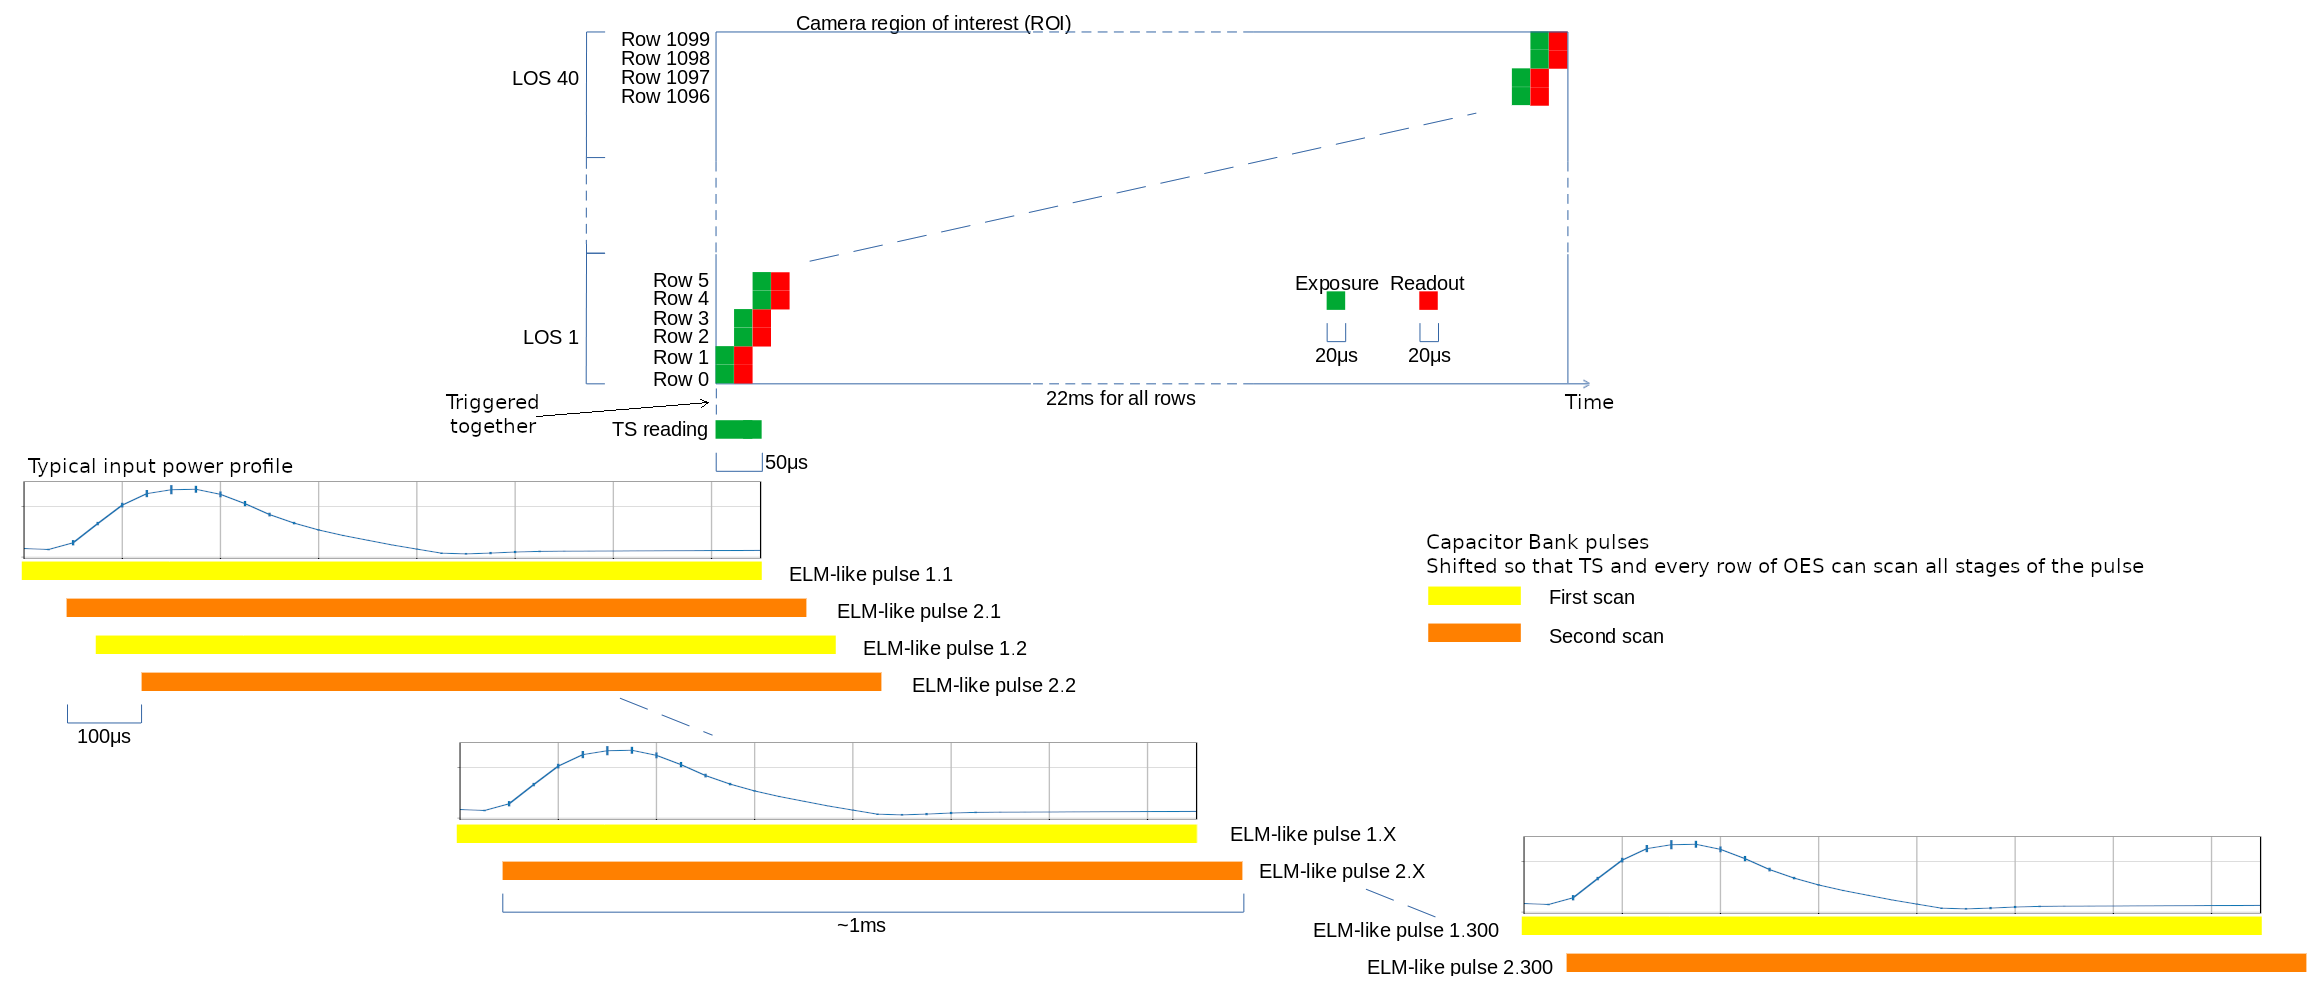
\includegraphics[width=\linewidth,trim={0 0 0 0},clip]{Chapters/chapter3/figs/sampling_strategy_2.png}
	\caption{Sampling strategy for TS and OES. At the top is indicated the progressive reading of the camera rows, with the integration time of TS is indicated. Below are each of the ELM-like. pulses. It is shown how the trigger of the capacitor bank is shifted in time and all the pulses are split in two scans. Dashed lines indicate an interruption of the space or time scale.}
	\label{fig:sampling1}
\end{figure*}

The rows are managed two at the time and during the readout of the rows $i-1/i$ the rows $i+1/i+2$ are exposed. Each OES LOS is composed of $\sim 24$ rows, so the time shift within would be $240\mu s$, much larger than the desired $50 \mu s$. Just below is indicated the TS integration time. OES and TS are synchronised such that the trigger to start data acquisition is sent to the two diagnostics simultaneously.
The time difference between CB and OES/TS trigger is initially such that OES and TS reading correspond to the end of the ELM-like pulse. From this the CB trigger is progressively delayed by $100\mu s$ so that TS and OES can acquire data about progressively earlier stages of the pulse.
For TS this sampling procedure returns directly $T_e$ and $n_e$ while for OES additional steps are required to: reconstruct frames with row data corresponding to the same time slice, bin the LOS, obtain the emission line brightness, calculate radial emissivity from the line integrates brightness. Further details are given in \autoref{OES data interpretation}. The final result is a map of the line emissivity in both space (radius) and time. The plasma is assumed poloidally symmetric with a radial coordinate of interval 1.06mm dictated by the OES resolution.

\section{OES data interpretation}\label{OES data interpretation}

\begin{figure}[!ht]
	\centering
	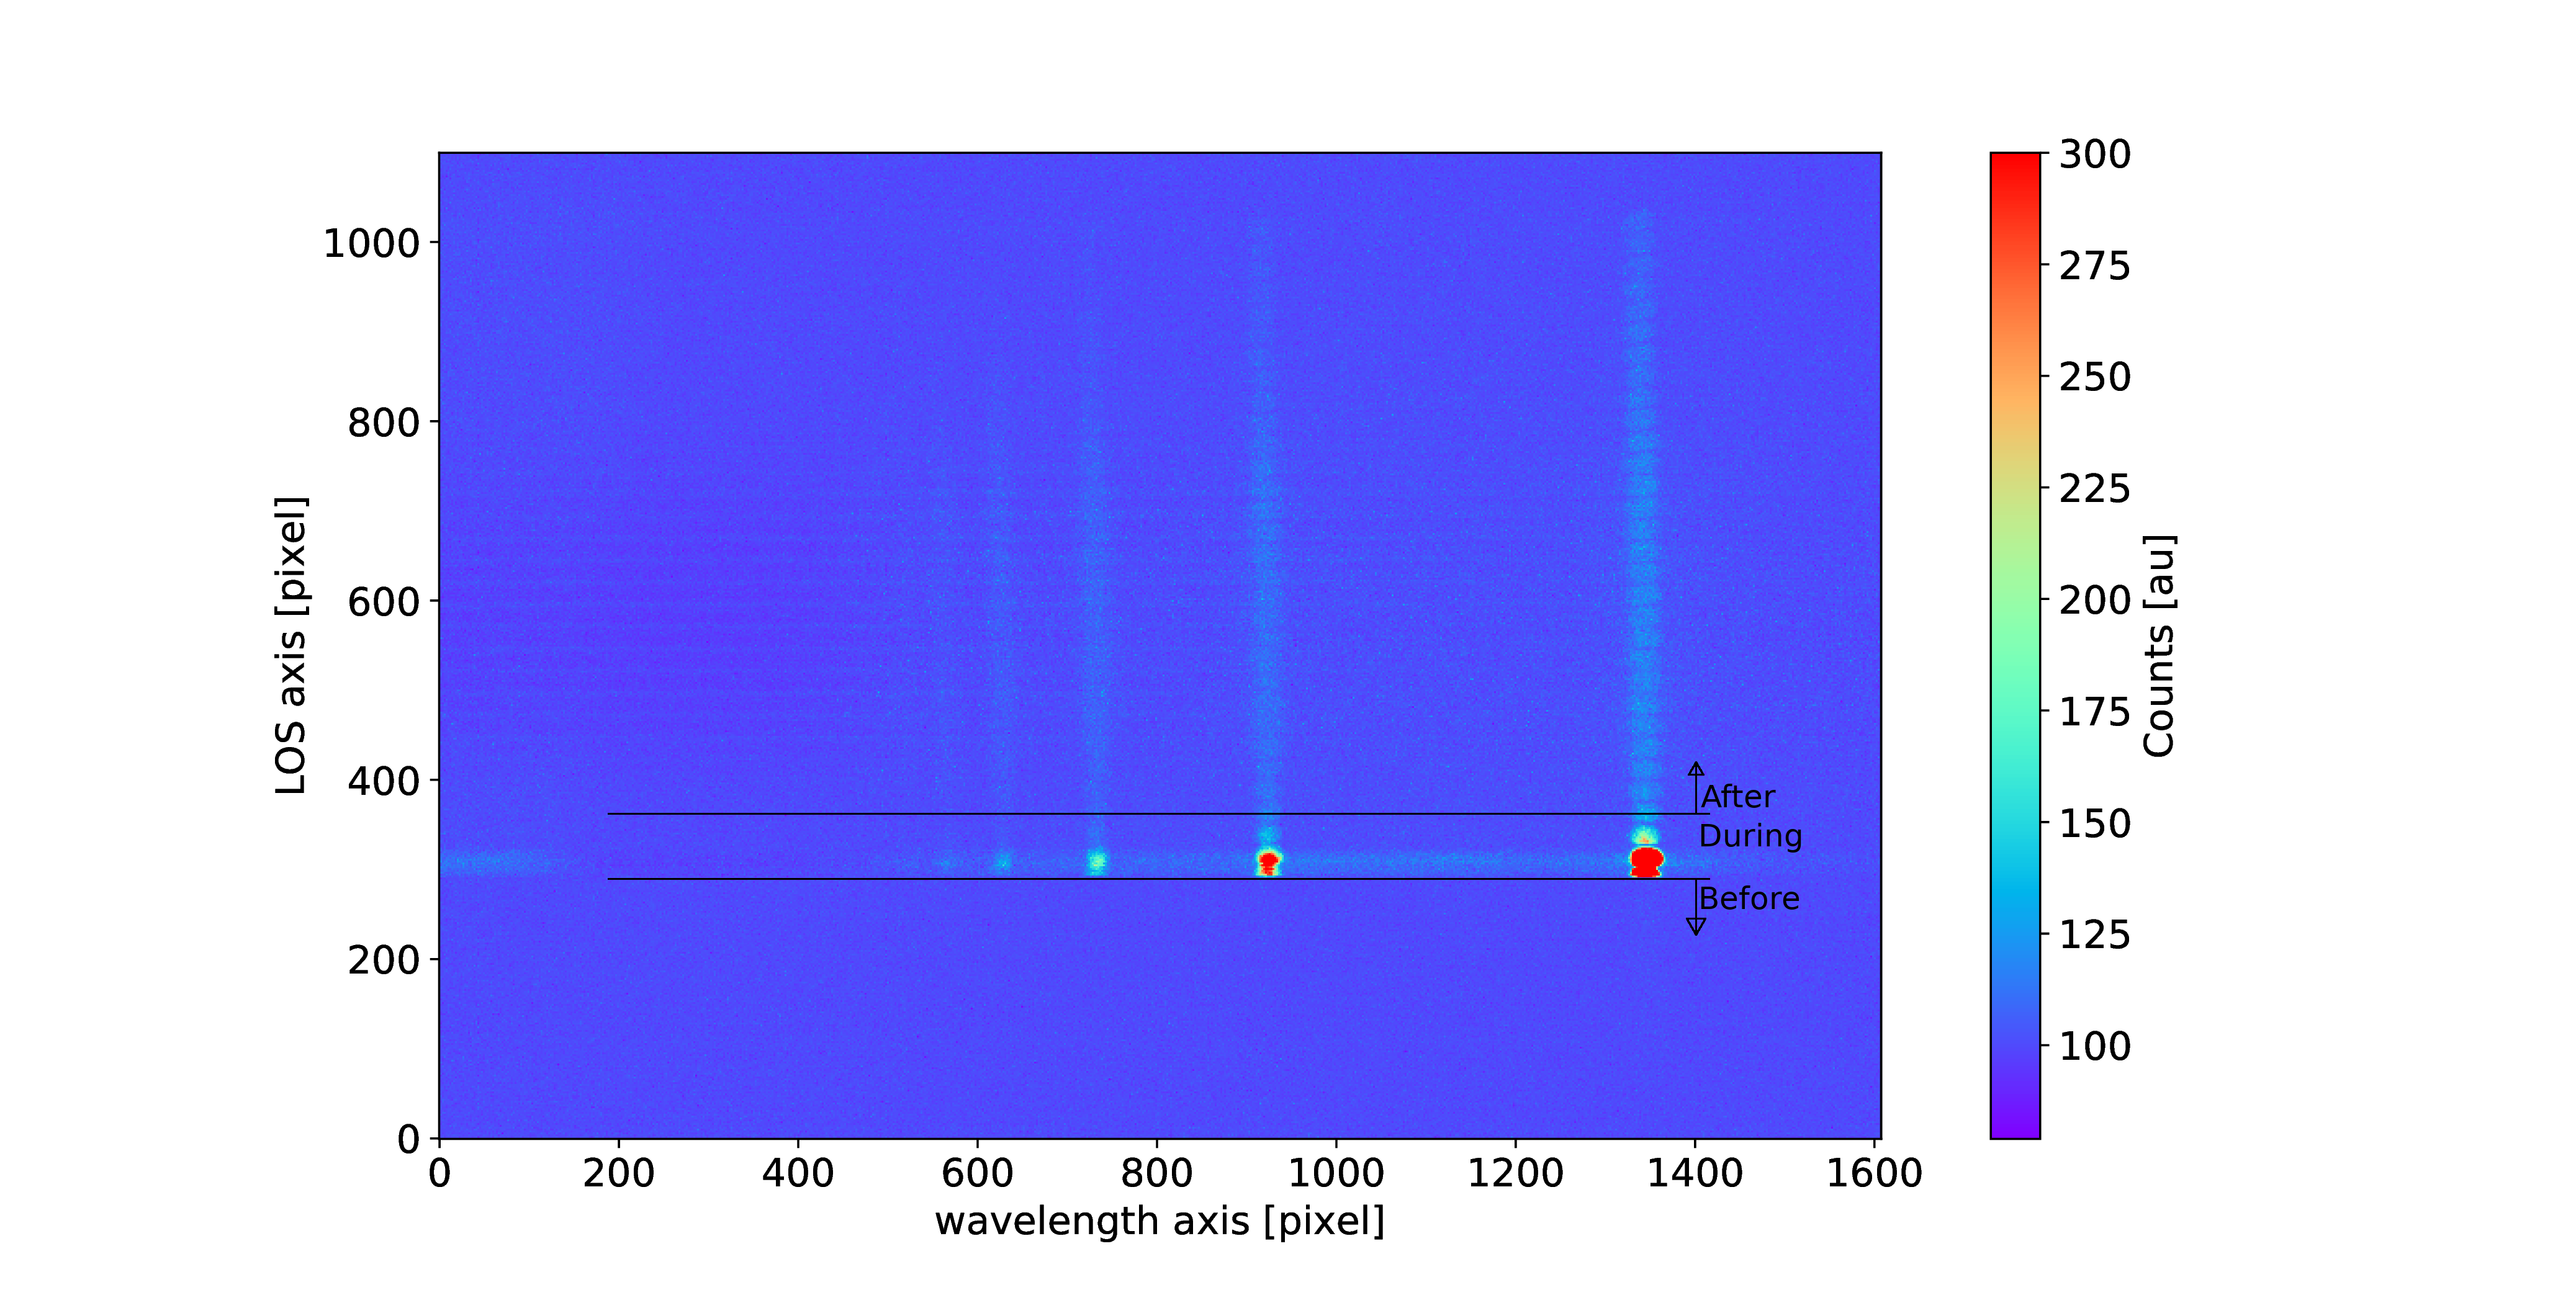
\includegraphics[width=0.7\linewidth,trim={440 50 600 150},clip]{Chapters/chapter3/figs/sample_oes.png}
	\caption{Example of a raw image from the OES. The readout starts from the bottom so higher rows represent later times. In the figure are indicated rows/times corresponding to different stages of the ELM-like pulse}
	\label{fig:sampling2}
\end{figure}

In this section it will be detailed how the OES measurements are processes to obtain the local radially and temporally resolved emissivity used to estimate the relevance of molecular processes.
The camera that was selected for the purpose of collecting time resolved OES data was a Photometrics Prime95B 25mm RM16C, because of the relatively high signal to noise in low light conditions and large size of the sensor. In \autoref{fig:sampling2} is shown the typical picture collected during an experiment when on top of a steady state plasma an ELM-like pulse is fired. The rows are read sequentially from the bottom, with a time shift equal to the integration time, minimum $20\mu s$. This means that for the particular example shown the rows indicated as \emph{Before} represent times before the effect of the ELM-like pulse propagated to the OES location. \emph{During} represents the pulse and \emph{After} is for times after the ELM-like pulse, characterised by homogeneous line emission from the hot gas filling the target chamber. From \autoref{fig:sampling2} it is also possible to distinguish part of the 40 line of sight that are available.

The first effect that is compensated is the sensitivity of the camera at low signal levels. The counts/light intensity correlation of the pixels is mostly linear, but deviates significantly below 6 counts and negative counts are returned at very low signal. A routine was developed to compensate for this thanks to dedicated measurements to find the correlation between light intensity and counts.

In order to decouple spatial and temporal information a scan is operated such that the ELM-like pulse is shifted in time respect to the start of the camera image record and TS measurement. More details on the sampling strategy in \autoref{Sampling strategy}. The presence of ELM-like pulses effected by capacitor bank misfires (see \autoref{Sampling strategy}) is found analysing the plasma source power and the data corresponding to those pulses is excluded. To separate the time and row dependency, for every row, column and time of interest the data in a range of $100\mu s$ and 8 rows is fit with a second degree polynomial in time and one in row. To avoid over smoothing the image a smaller weight is assigned for increasing times and row difference from the one that is being examined. In \autoref{fig:sampling3} is shown the time/row decoupled image. The output time step has a $50\mu s$ resolution to match TS data.

\begin{figure}[!ht]
	\centering
	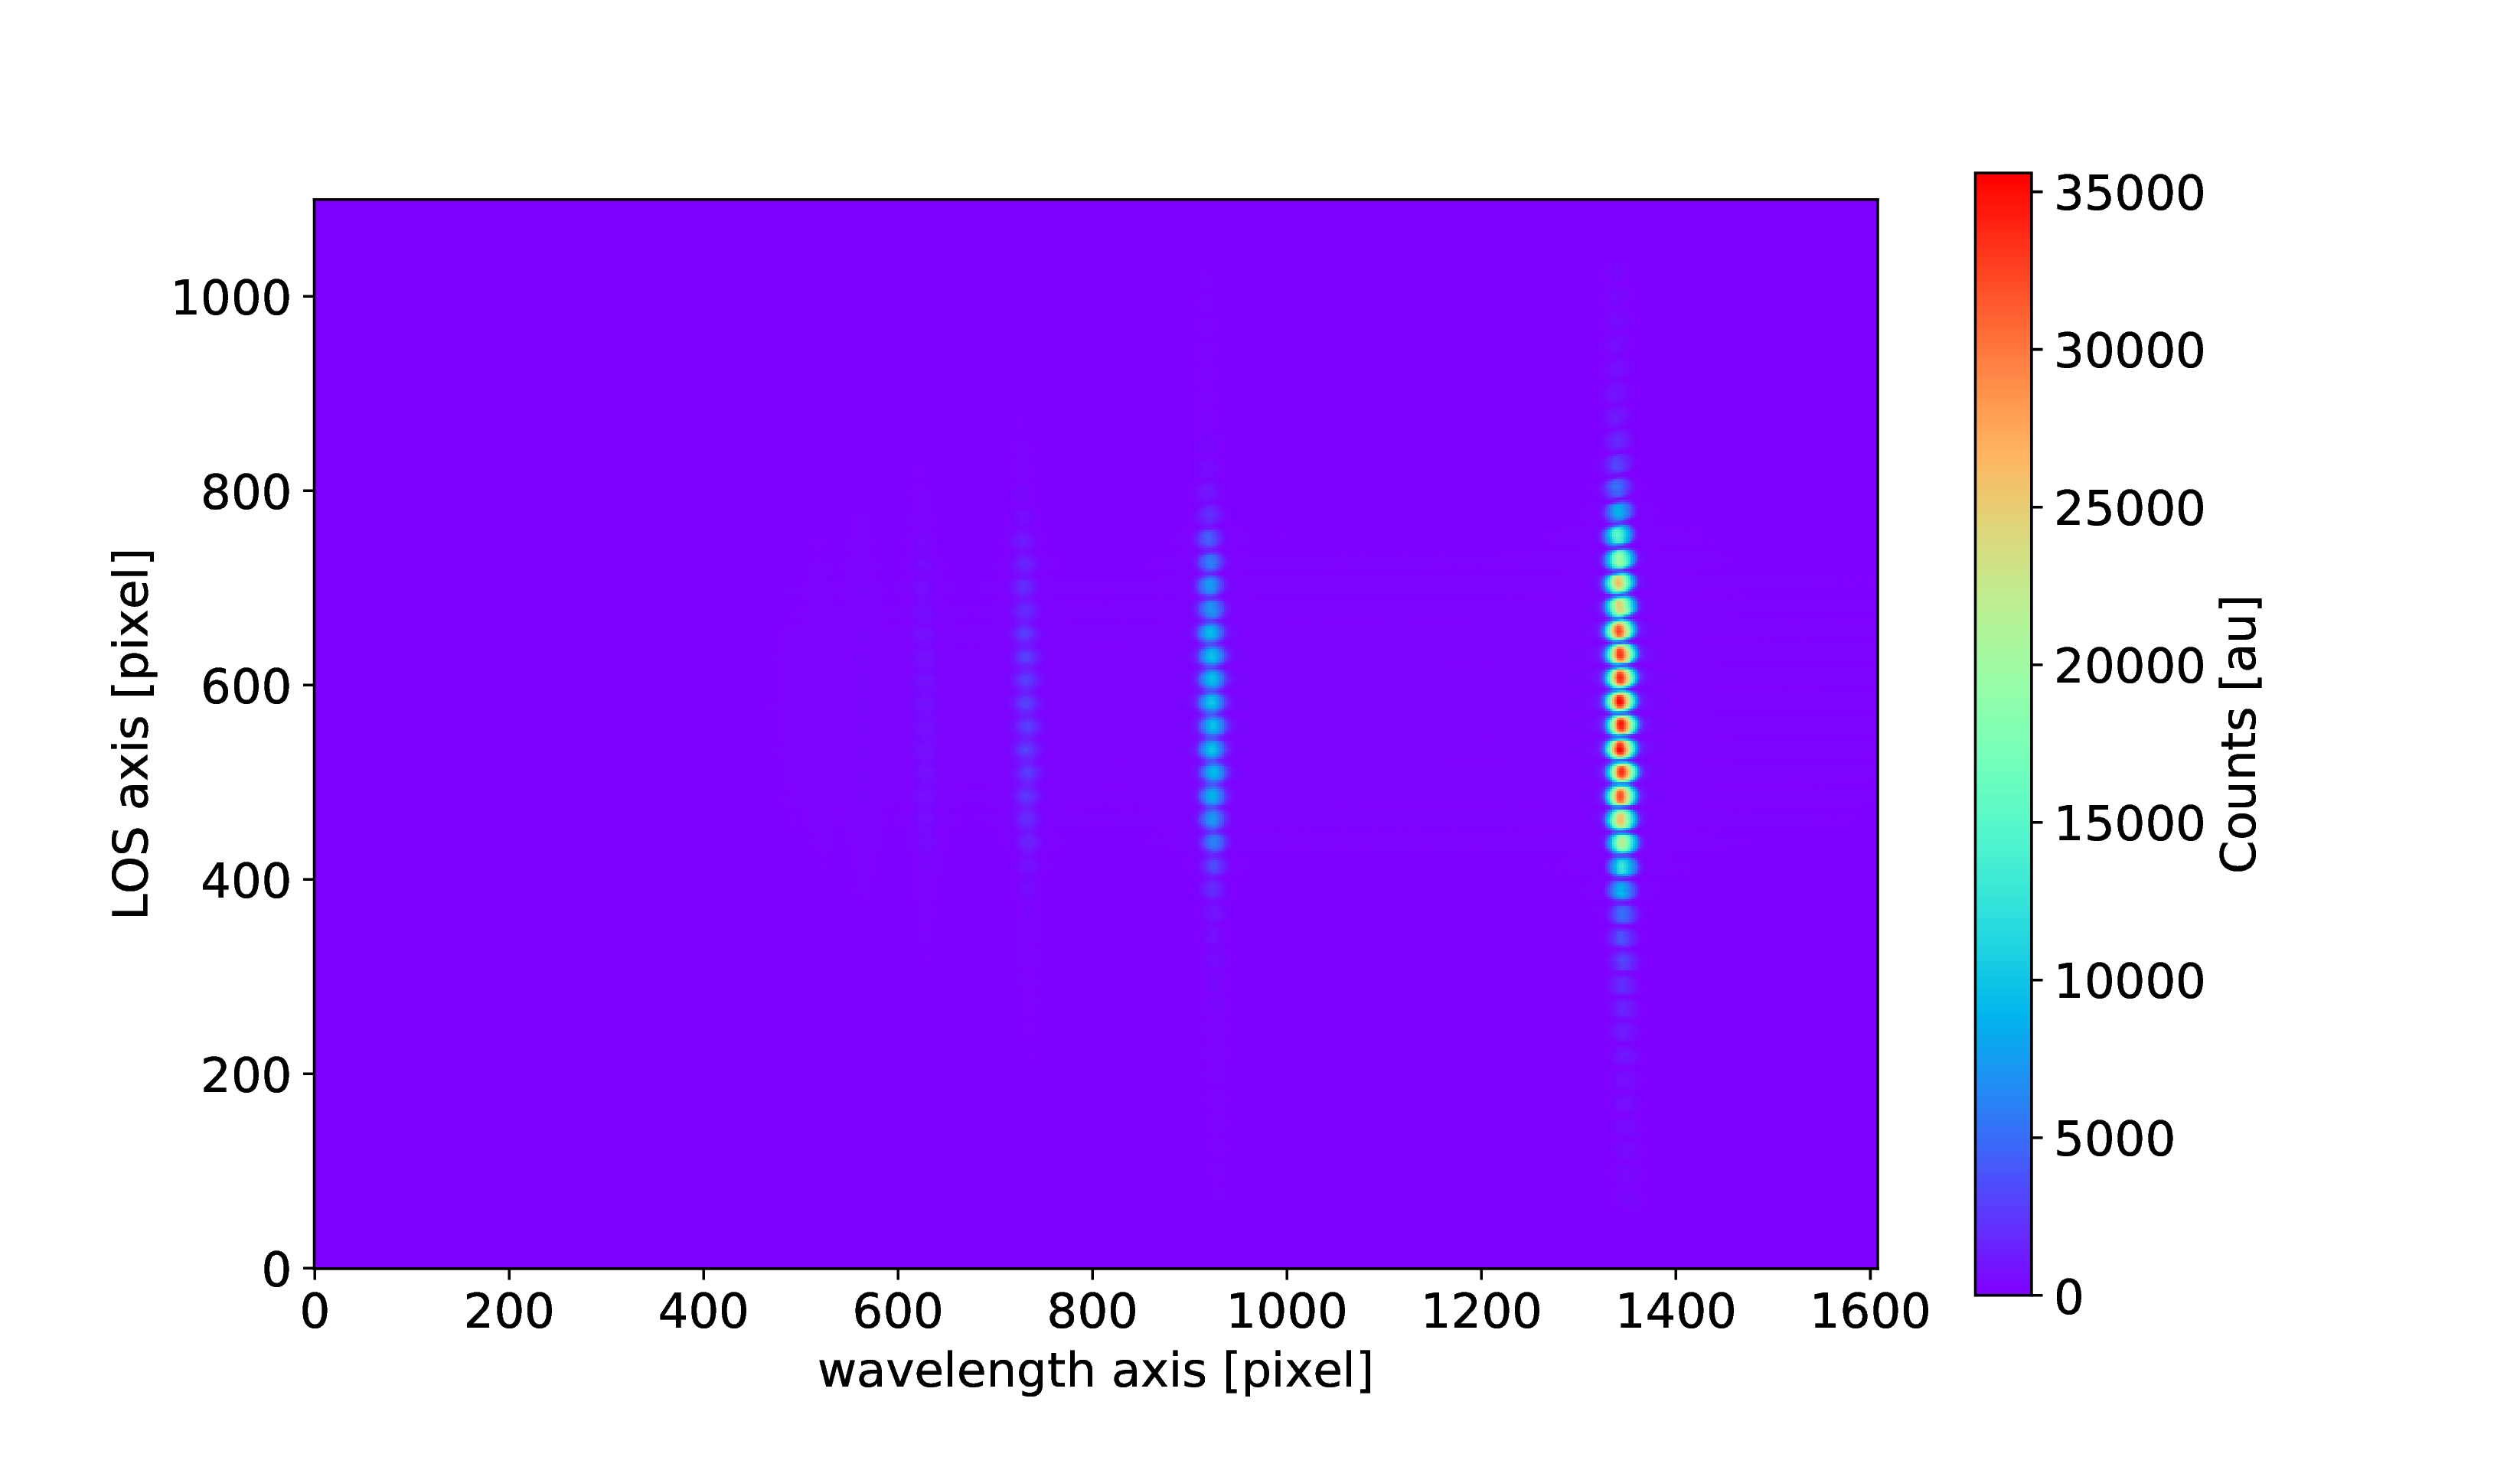
\includegraphics[width=0.7\linewidth,trim={100 30 290 200},clip]{Chapters/chapter3/figs/sample_oes2.png}
	\caption{Example of decomposed time frame showing the symmetry of the image to the vertical pixel $\sim$600, likely representing the location of the plasma column axis.}
	\label{fig:sampling3}
\end{figure}

The counts are summed among the rows composing each LOS and the line intensity is calculated by integrating above the background level. Brightness is then converted to emissivity via Abel inversion. The line emission is supposed poloidally symmetric and the plasma optically thin. In order to avoid unrealistic discontinuities given by noise, the superimposition of 3 Gaussian is fitted to the brightness profile as done by Barrois.\cite{Science2017} Each Gaussian can then be Abel inverted analytically and summed to obtain the total emissivity. In this process the uncertainties are propagated to be used in subsequent steps in the analysis. An example of the inversion process is shown in \autoref{fig:sampling4}. Given the signal to noise ratio and the available lines it is decided to use Balmer lines $p=4-8 \rightarrow 2$.

\begin{figure}[!ht]
     \centering
     \begin{subfigure}{0.8\linewidth}
         \centering
         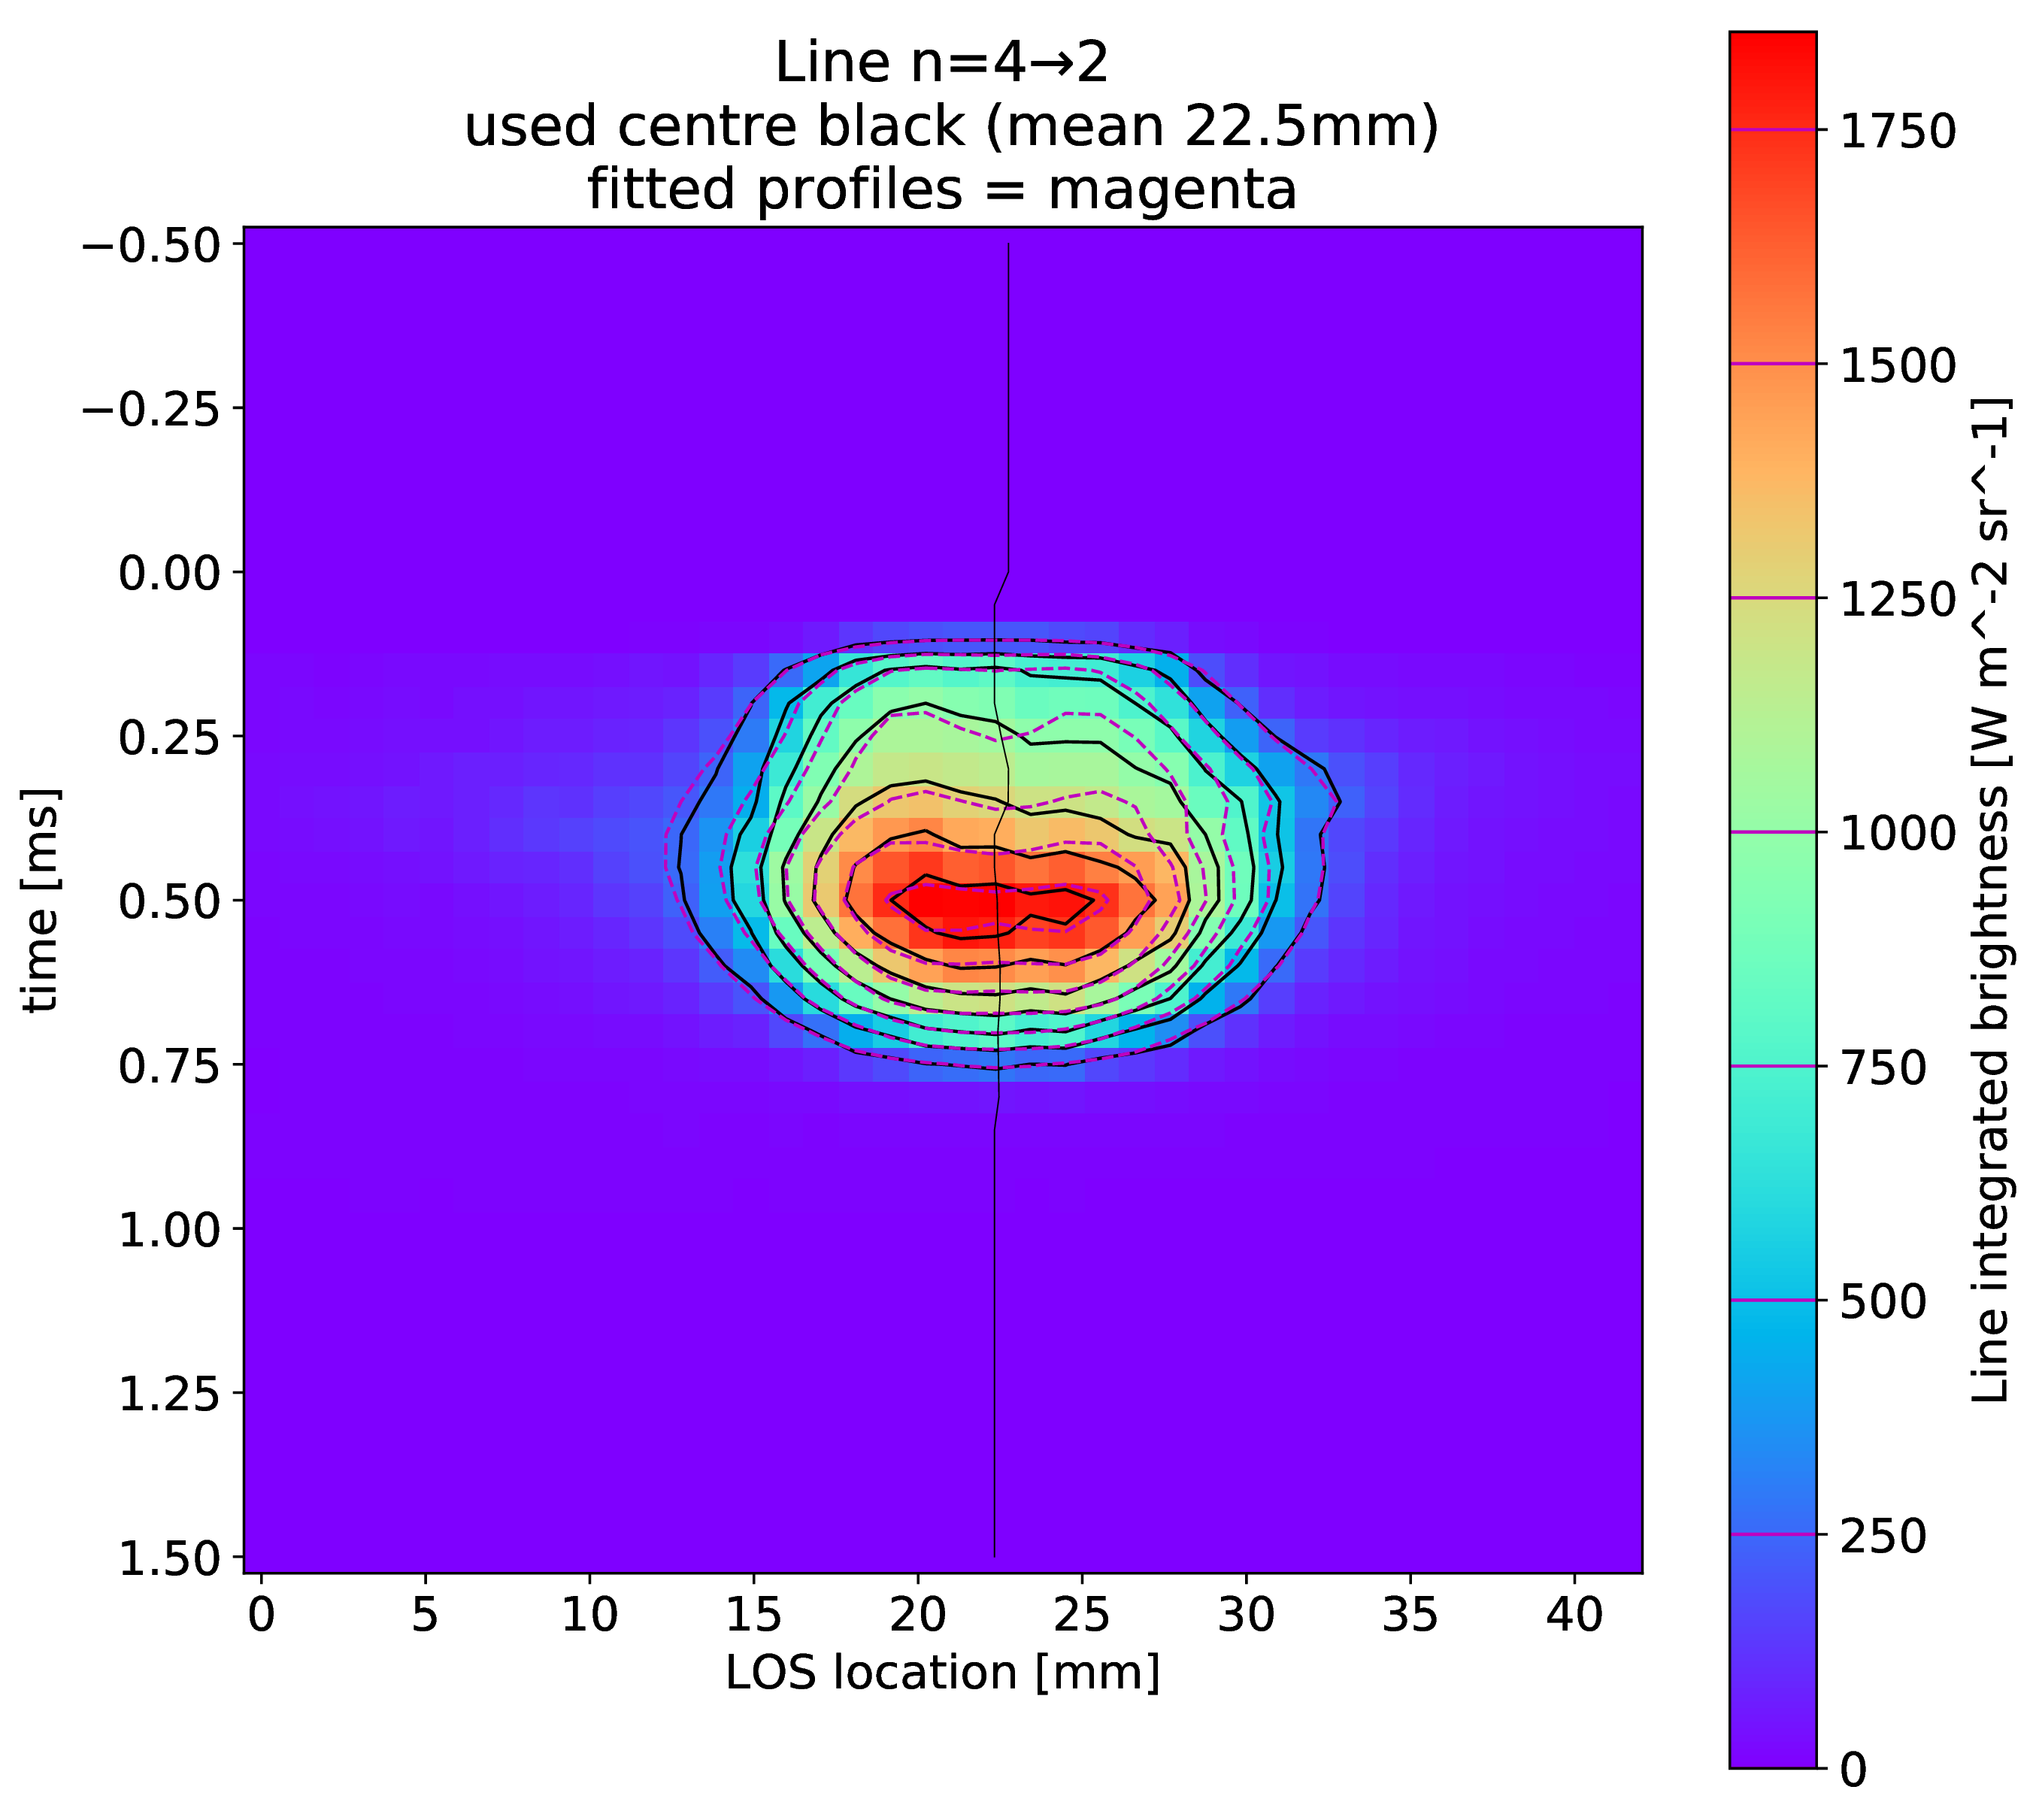
\includegraphics[width=0.7\textwidth,trim={20 170 550 300},clip]{Chapters/chapter3/figs/line_integrted_profile4.png}
         % \vspace*{-8mm}
         \caption{OES line integrated brightness}
         \label{fig:sampling4a}
         %{\color{white}\caption{\phantom{wew}}\label{fig:TSa}}
     \end{subfigure}
     % \hfill
     \begin{subfigure}{0.14\linewidth}
         % \centering
         \vspace*{-10mm}
         \hspace*{-20mm}
         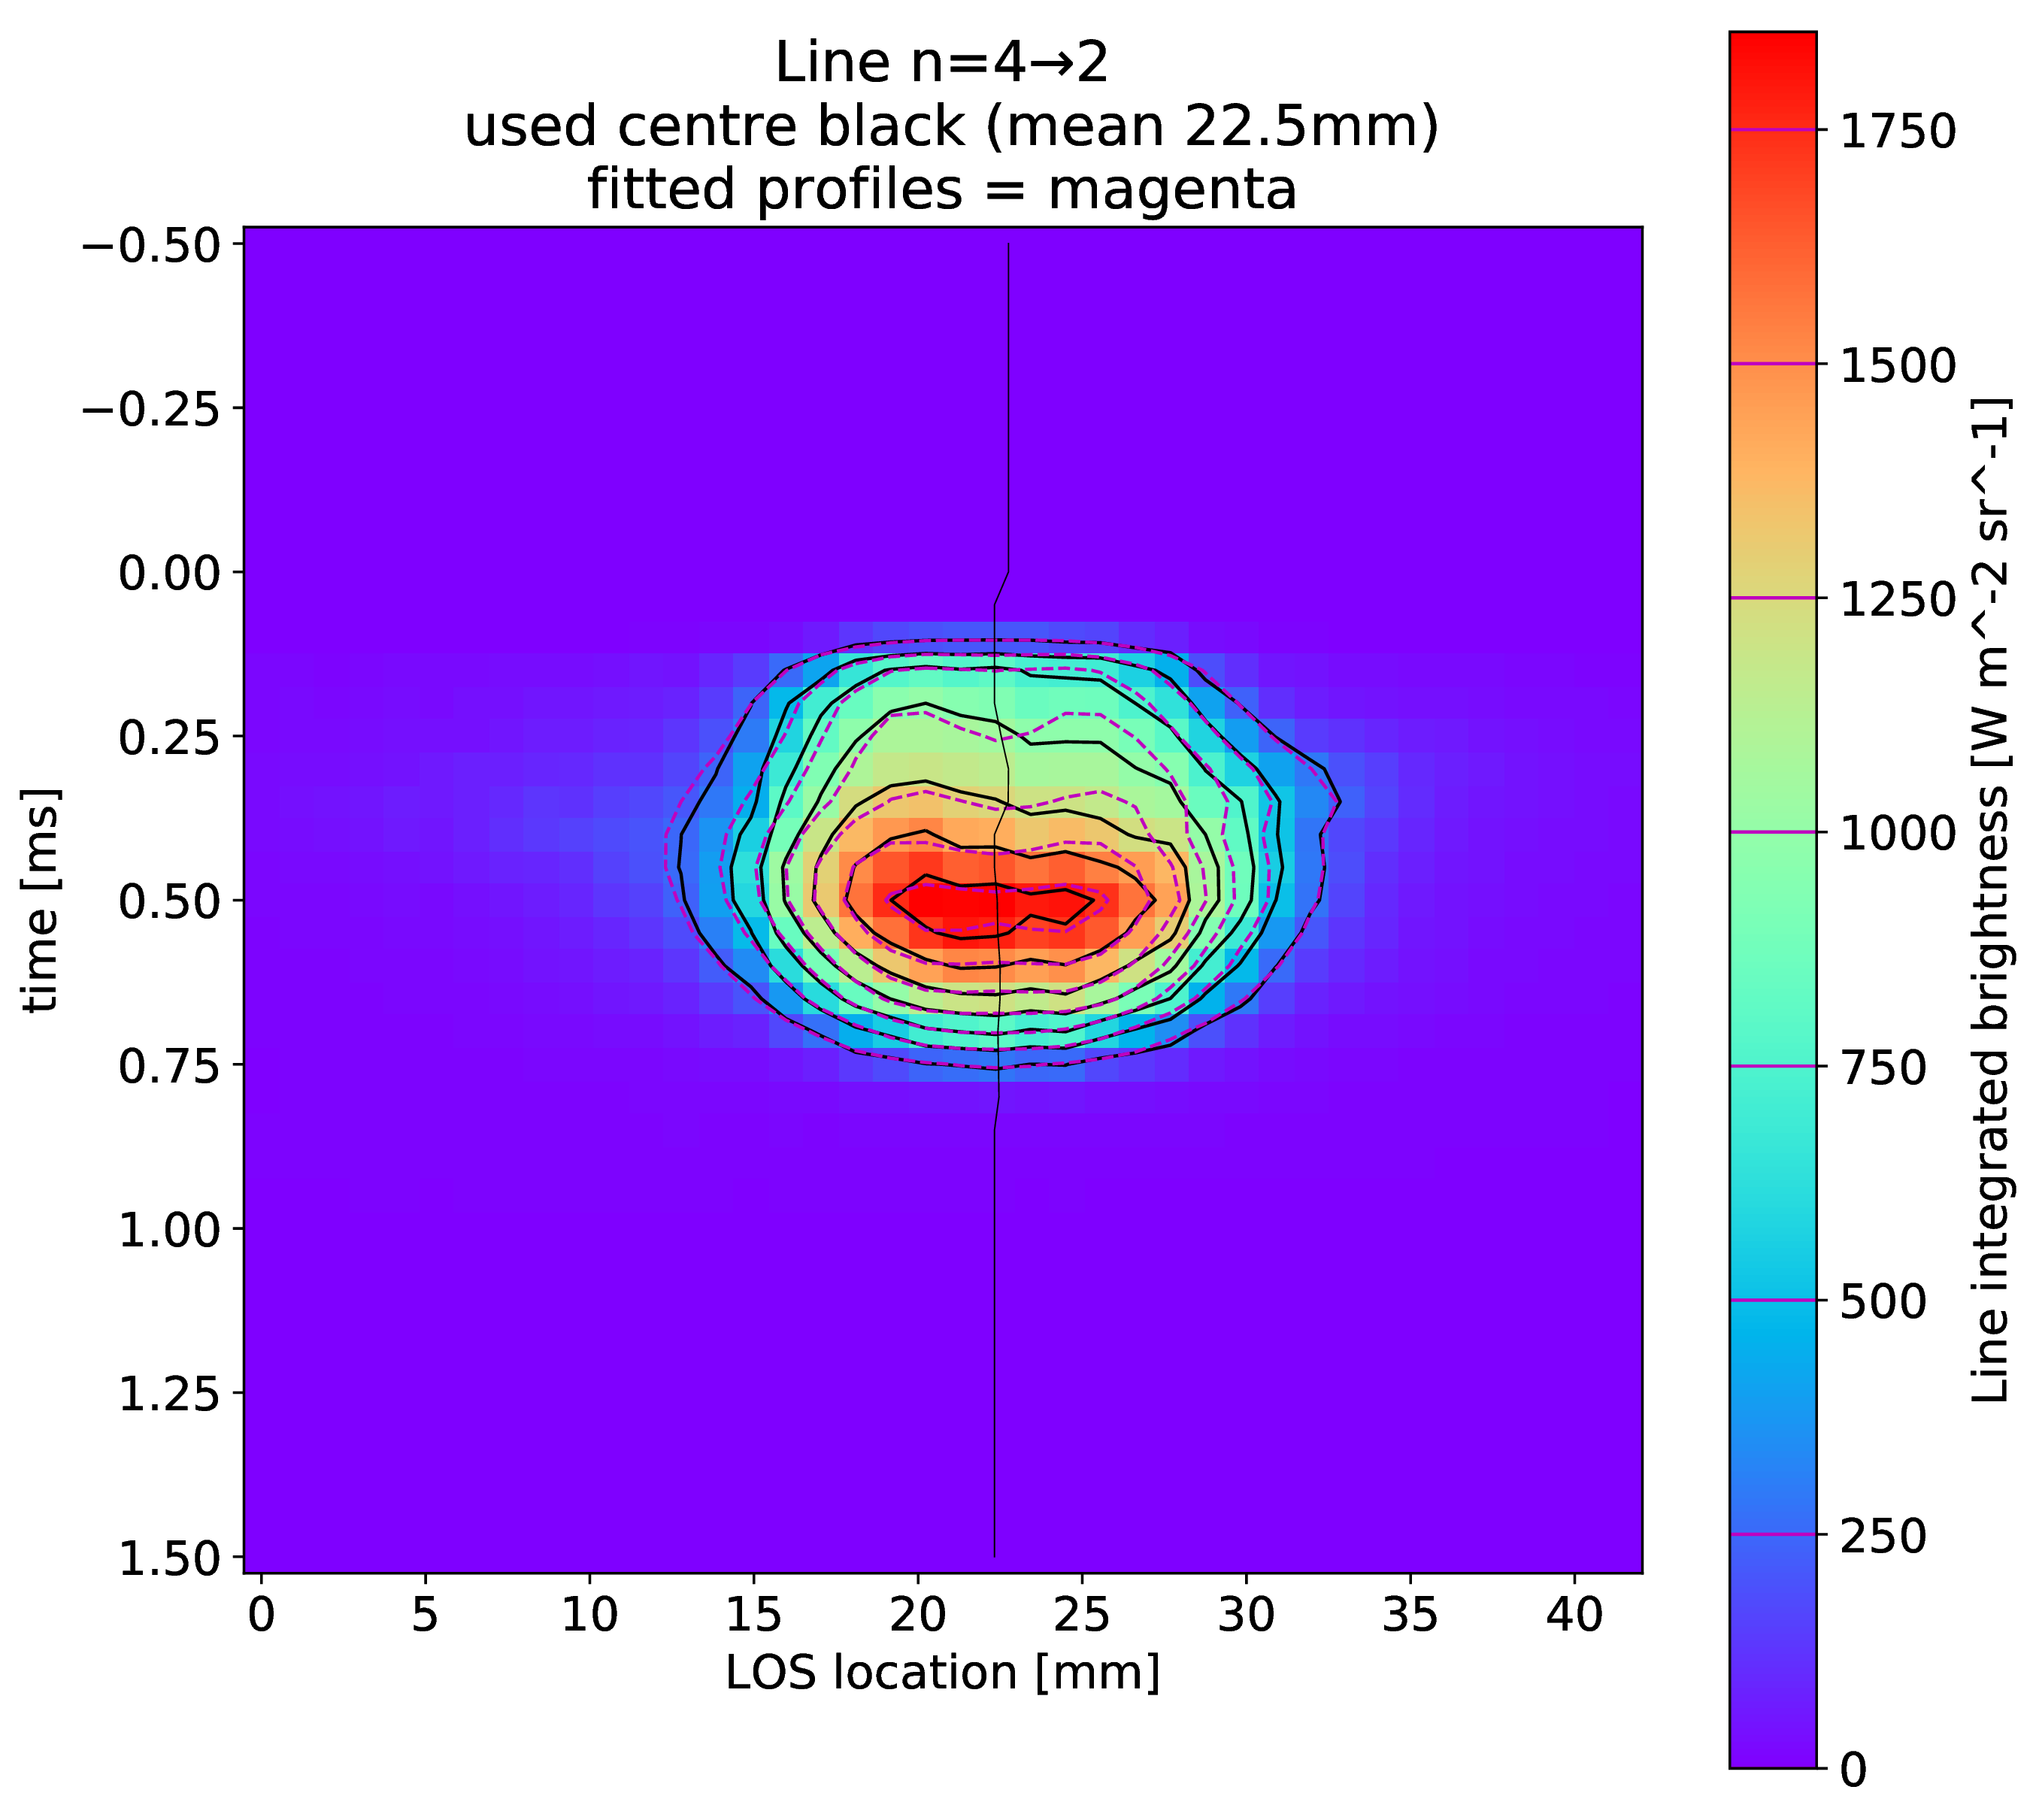
\includegraphics[width=0.7\textwidth,trim={2200 0 0 40},clip]{Chapters/chapter3/figs/line_integrted_profile4.png}
         % \vspace*{-8mm}
         % \caption{Line integrated brightness}
         % \label{fig:sampling4a}
         %{\color{white}\caption{\phantom{wew}}\label{fig:TSa}}
     \end{subfigure}
     % \hfill
     \begin{subfigure}{0.8\linewidth}
         \centering
         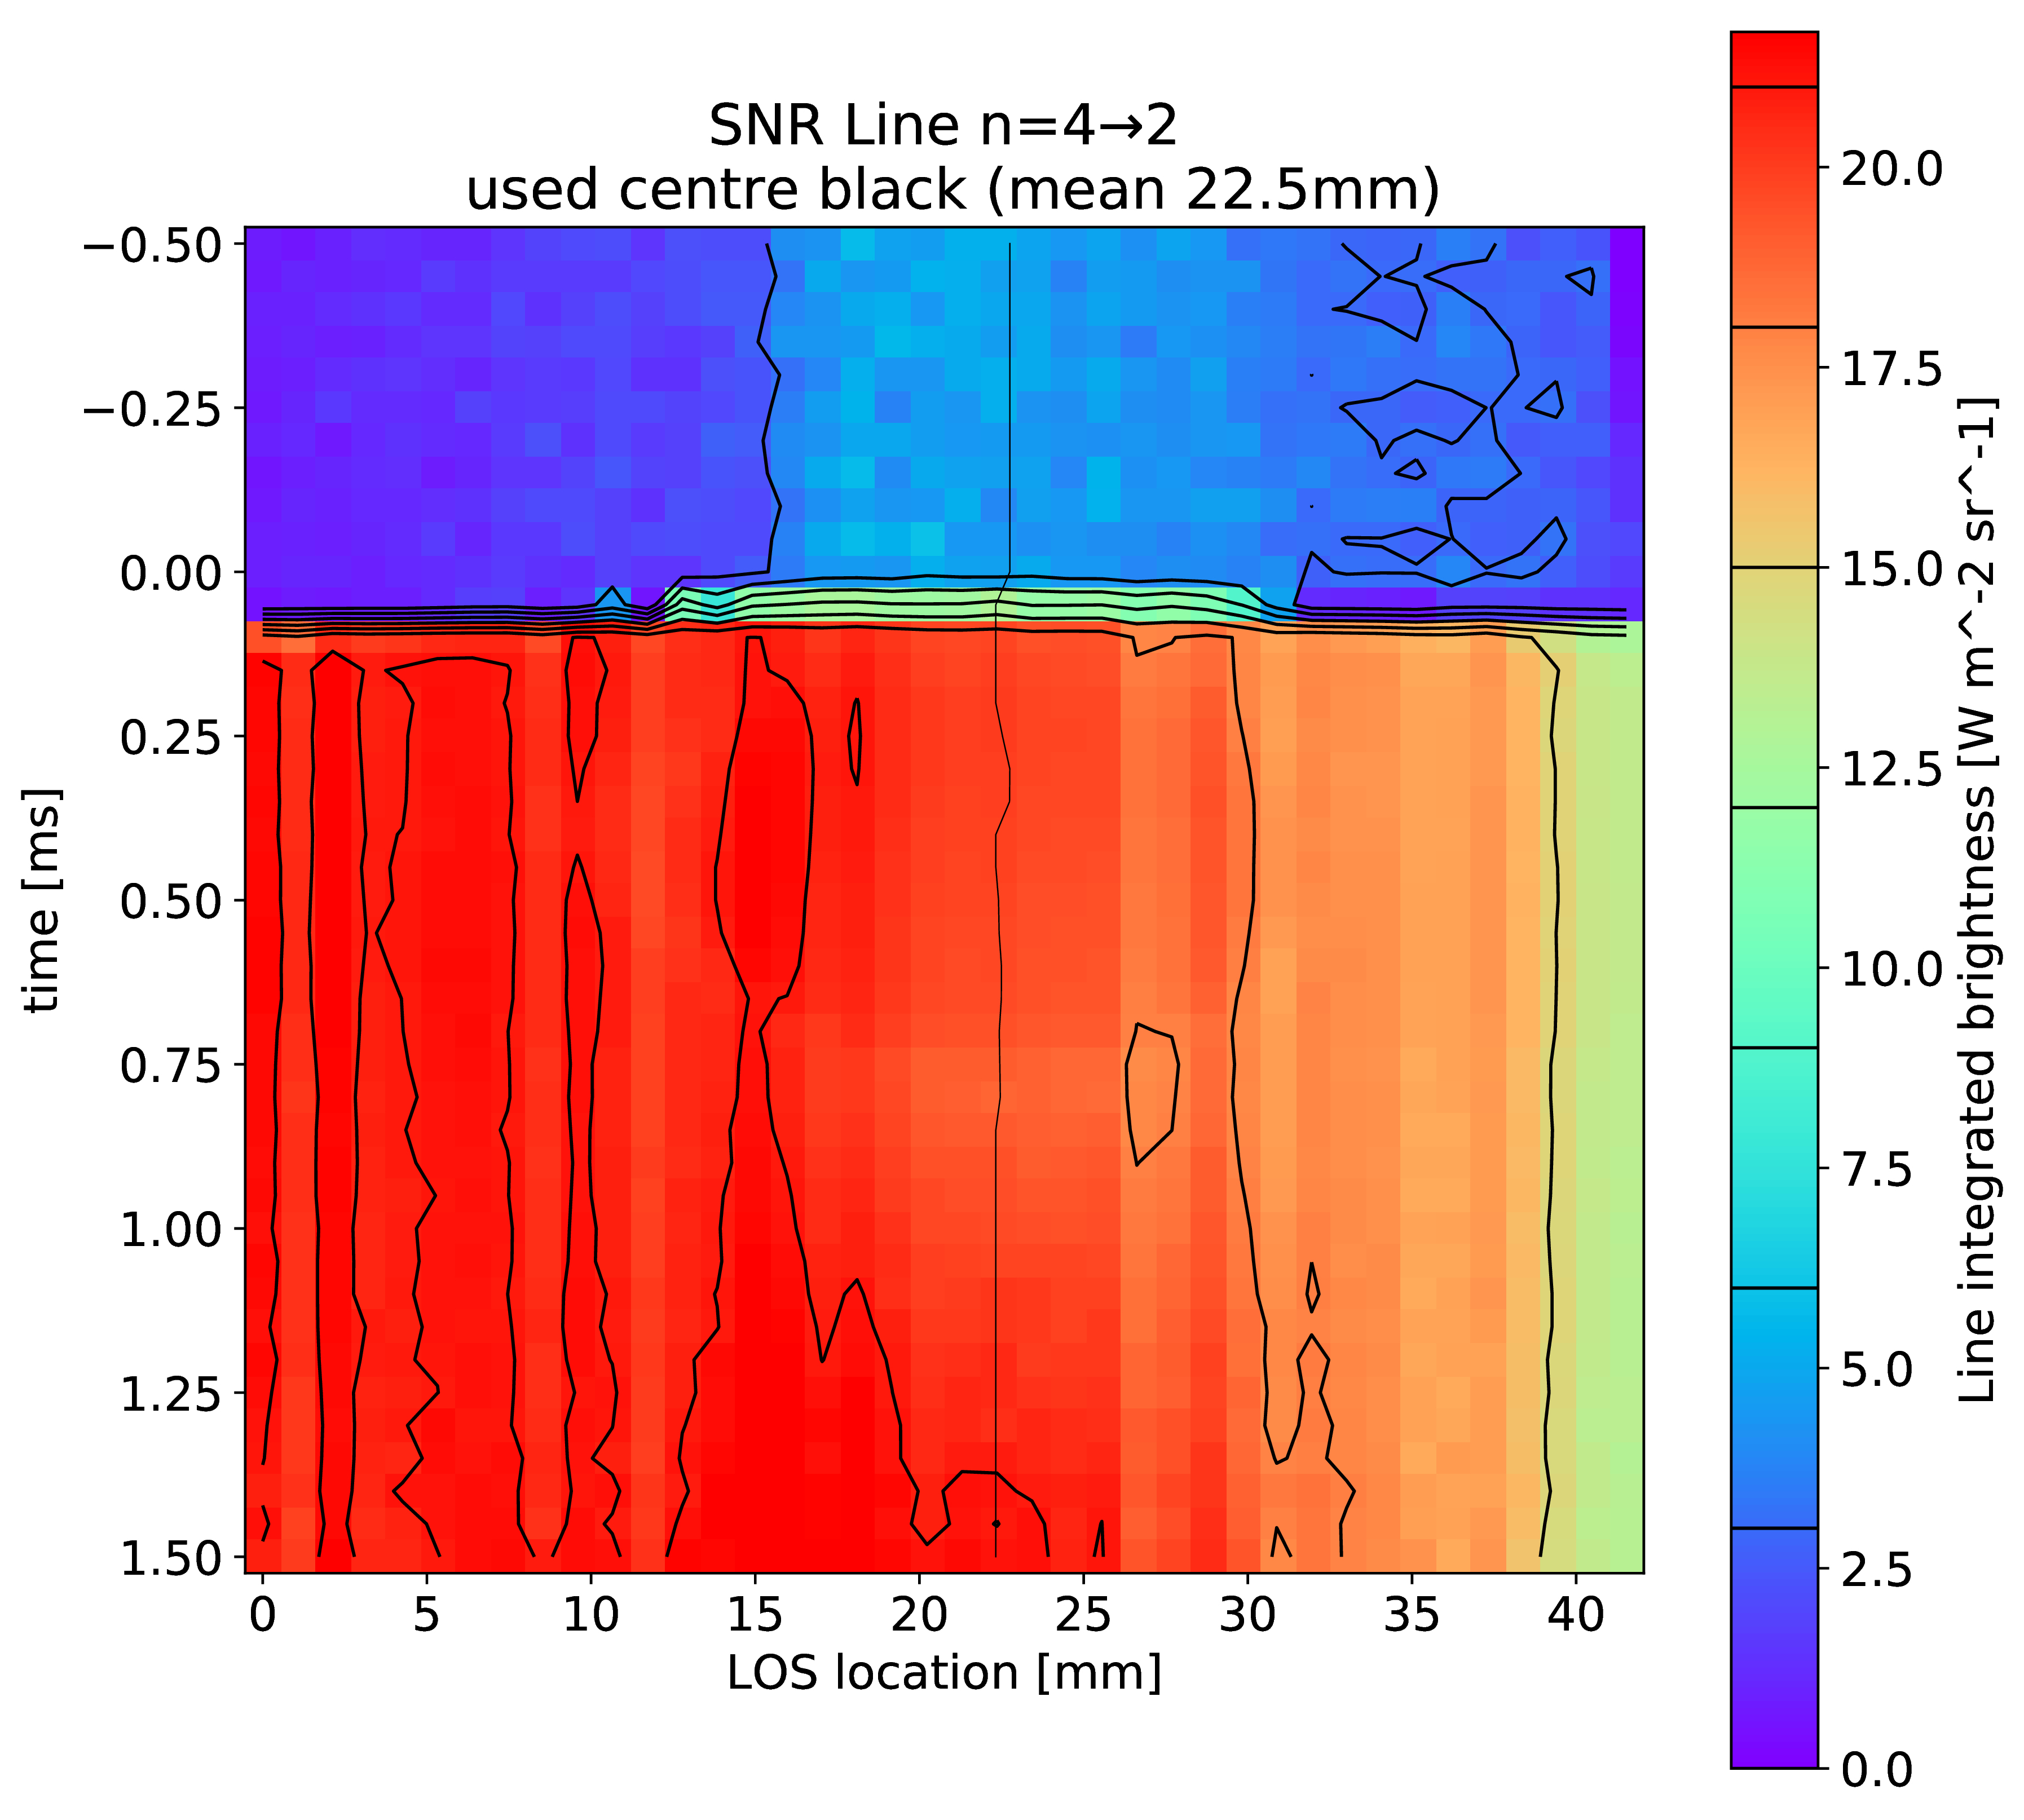
\includegraphics[width=0.7\textwidth,trim={20 220 650 400},clip]{Chapters/chapter3/figs/line4SNR.jpg}
         % \vspace*{-8mm}
         \caption{OES line integrated brightness SNR}
         \label{fig:sampling4b}
         %{\color{white}\caption{\phantom{wew}}\label{fig:TSb}}
     \end{subfigure}
     % \hfill
     \begin{subfigure}{0.095\linewidth}
         % \centering
         \vspace*{-10mm}
         \hspace*{-20mm}
         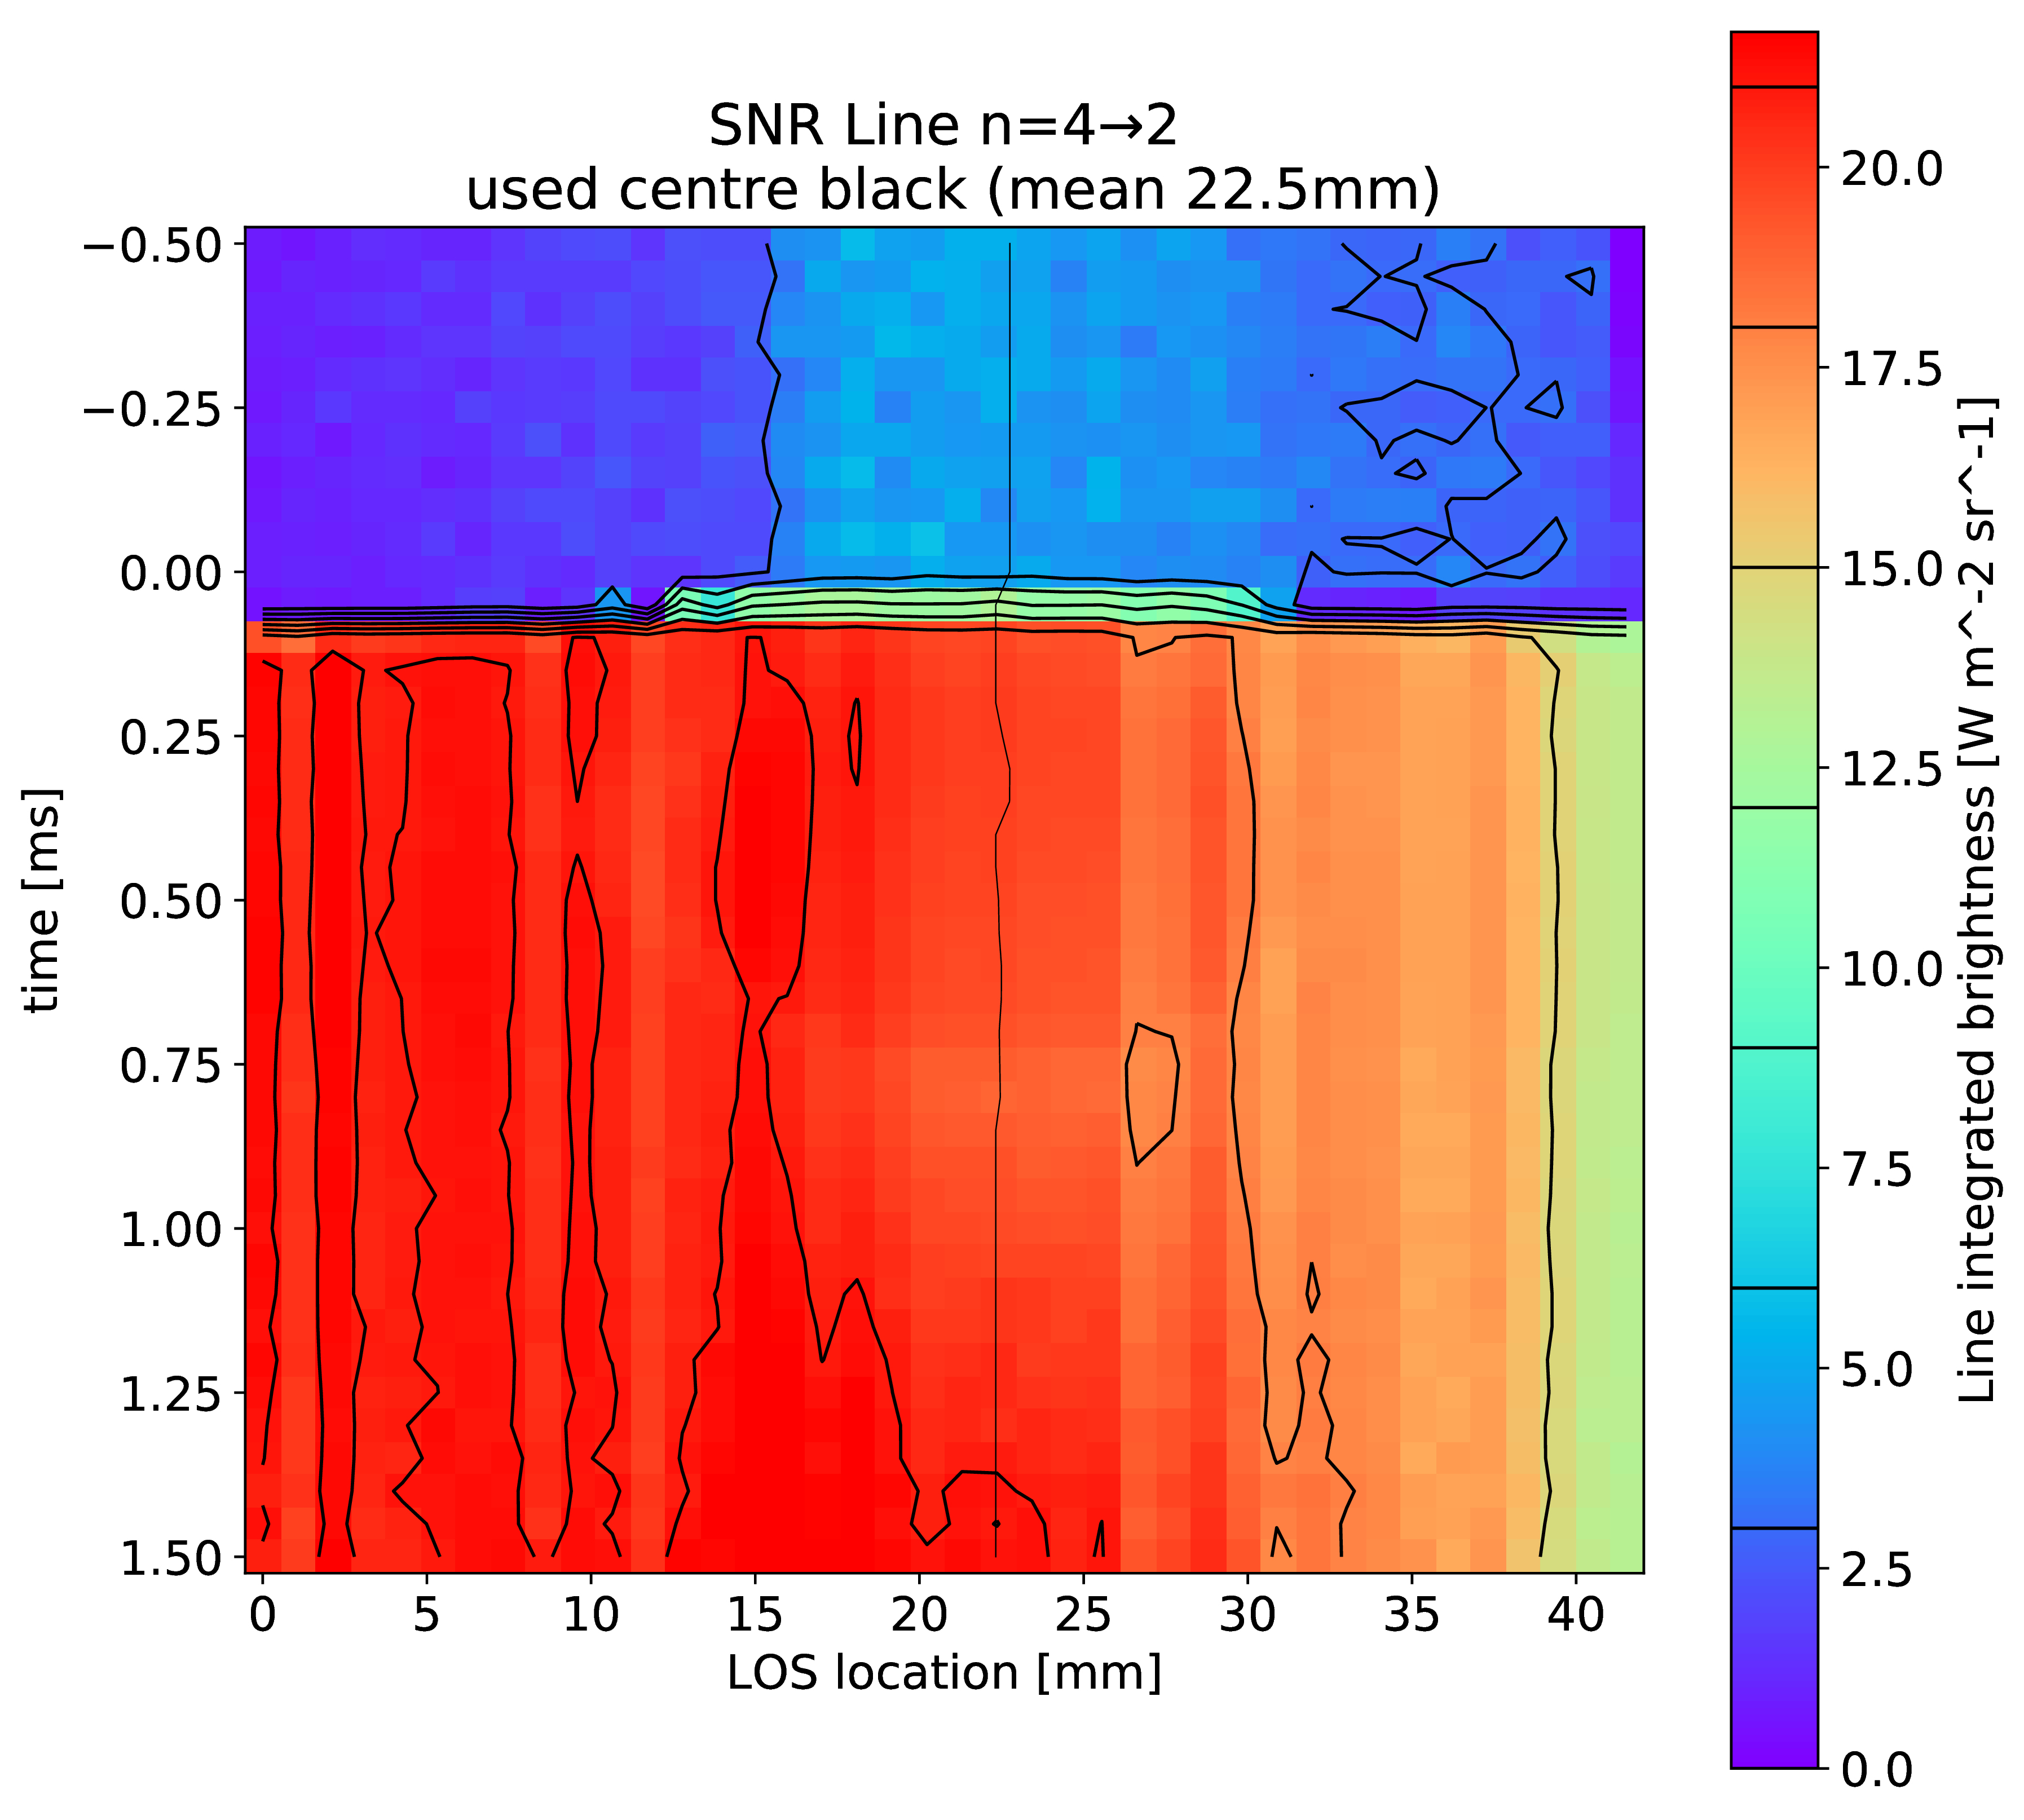
\includegraphics[width=0.7\textwidth,trim={3000 0 125 40},clip]{Chapters/chapter3/figs/line4SNR.jpg}
         % \vspace*{-8mm}
         % \caption{Line integrated brightness}
         % \label{fig:sampling4a}
         %{\color{white}\caption{\phantom{wew}}\label{fig:TSa}}
     \end{subfigure}
        \caption{(\subref{fig:sampling4a}): example of a fit of the OES line integrated brightness and relative SNR with 3 Gaussians for the $n=4\rightarrow 2$ line. In magenta the profile of the fitted Gausinass, in thin black the found location of the plasma column centre. (\subref{fig:sampling4b}): SNR of the line integrated brightness.}
        \label{fig:sampling4}
\end{figure}


\section{Target temperature profile interpretation}\label{Target temperature profile interpretation}
In this section the mathematical models used in the interpretation of the target temperature data will be examined in more detail.

The heat delivered by the plasma to the target during an ELM-like pulse is shaped in time and space. The power density is spatially peaked at the centre of the plasma beam due to the peak in plasma density and temperature. It temporally follows the power evolution dictated by the discharge of the capacitor bank as measured by the plasma source (see \autoref{fig:TS1} for an example). The full spatial and temporal power density distribution of the target heat source is difficult to obtain from the surface temperature for all experimental conditions but analytical solutions that can approximate the peak temperature are available. As mentioned in \autoref{IR camera} the ones considered in this work are:

\begin{itemize}
\item[Model1] a temporally square heat wave delivered uniformly on a semi infinite plane: the surface temperature increase in the heating and cooling phases are respectively\cite{Behrisch1980}
\begin{equation}
\label{eq:square1}
\begin{aligned}
{\Delta T(t)}_r &= F_0 \frac{2}{ \sqrt{\pi \rho c_p k }} \lbrace { \sqrt{t-t_0} } \rbrace = \frac{E_0}{\tau} \frac{2}{ \sqrt{\pi \rho c_p k }} \lbrace { \sqrt{t-t_0} } \rbrace \\ {\Delta T(t)}_c &= F_0 \frac{2}{ \sqrt{\pi \rho c_p k} } \lbrace { \sqrt{t-t_0} - \sqrt{t-t_0 - {\tau}} } \rbrace
\end{aligned}
\end{equation}
with $\tau$ the duration of the heat pulse and $t_0$ its start, $F_0$ the peak power density, $E_0$ the energy density, $\rho$ the density, $c_p$ the specific heat capacity and $k$ the thermal conductivity
\item[Model2] a temporally square heat wave delivered by a spatially Gaussian beam: the surface temperature evolution in the heating and cooling phases are respectively\cite{Bauerle2011}
\begin{equation}
\label{eq:square2}
\begin{aligned}
{\Delta T(t)}_r &= \frac{2}{\pi} {\Theta}_c \tan^{ -1}(2 \sqrt{ \tilde{t}} ) 
\\ 
{\Delta T(t)}_c &= \frac{2}{\pi} {\Theta}_c \tan^{ -1} \left( \frac{2 \sqrt{ \tilde{t}} - 2 \sqrt{ \tilde{t} - \tilde{\tau} }}{ 1+4 \sqrt{ \tilde{t}} \sqrt{ \tilde{t} - \tilde{\tau} }} \right)
\end{aligned}
\end{equation}
with
\begin{equation}
\label{eq:square3}
\begin{aligned}
{\Theta}_c = \frac{\sqrt{\pi}}{2} \frac{F_0 {\omega}_0}{k} , \tilde{t} = \frac{(t-t_0) D}{{\omega}_0} , \tilde{\tau} = \frac{\tau D}{{\omega}_0} , D = \frac{k}{ \rho c_p }
\end{aligned}
\end{equation}
and $\omega_0$ the $1/e$ size of the spatial heat distribution on the target
\item[Model3] a temporally triangular heat wave delivered by a spatially Gaussian beam: the surface temperature evolution in the heat rise, heat decreasing and cooling phases are respectively
% \begin{equation}
% \label{eq:triang}
% \begin{aligned}
% {\Delta T(t)}_r = \frac{2}{\pi} {\Theta}_c \frac{1}{\tilde{\tau_r}}   \left\{ {\tilde{t}} \tan^{ -1}(2 \sqrt{ \tilde{t}} )  \frac{-1}{4} [ 2 \sqrt{ \tilde{t}} - \tan^{ -1}(2 \sqrt{ \tilde{t}} ) ] \right\}
% \\ 
% {\Delta T(t)}_d = {\Delta T(t)}_r - \frac{2}{\pi} {\Theta}_c \left( \frac{1}{\tilde{\tau_r}} +\frac{1}{\tilde{\tau_d}}  \right) \left\{ {(\tilde{t} - \tilde{\tau_r})} \tan^{ -1} (2 \sqrt{ \tilde{t} - \tilde{\tau_r}} ) + \right. \\ \left. - \frac{1}{4 } [ 2 \sqrt{ \tilde{t} - \tilde{\tau_r}} - \tan^{ -1}(2 \sqrt{ \tilde{t} - \tilde{\tau_r}} ) ] \right\} 
% \\ 
% {\Delta T(t)}_c = {\Delta T(t)}_d + \frac{2}{\pi} {\Theta}_c \frac{1}{\tilde{\tau_d}} \left\{ {(\tilde{t} - \tilde{\tau_r} - \tilde{\tau_d})} \tan^{ -1}(2 \sqrt{ \tilde{t} - \tilde{\tau_r} - \tilde{\tau_d}} )+ \right. \\ \left. - \frac{1}{4 } [ 2 \sqrt{ \tilde{t} - \tilde{\tau_r} - \tilde{\tau_d}} - \tan^{ -1}(2 \sqrt{ \tilde{t} - \tilde{\tau_r} - \tilde{\tau_d}} ) ] \right\} 
% \end{aligned}
% \end{equation}


\begin{equation}
\label{eq:triang}
\begin{aligned}
{\Delta T(t)}_r &= \frac{2}{\pi} {\Theta}_c \frac{1}{\tilde{\tau_r}}   \left\{ {\tilde{t}} \tan^{ -1}(2 \sqrt{ \tilde{t}} )  \frac{-1}{4} [ 2 \sqrt{ \tilde{t}} - \tan^{ -1}(2 \sqrt{ \tilde{t}} ) ] \right\}
\\ 
{\Delta T(t)}_d &= {\Delta T(t)}_r - \frac{2}{\pi} {\Theta}_c \left( \frac{1}{\tilde{\tau_r}} +\frac{1}{\tilde{\tau_d}}  \right) \left\{ {(\tilde{t} - \tilde{\tau_r})} \tan^{ -1} (2 \sqrt{ \tilde{t} - \tilde{\tau_r}} )  \right. 
\\
& \phantom{+} \left. - \frac{1}{4 } [ 2 \sqrt{ \tilde{t} - \tilde{\tau_r}} - \tan^{ -1}(2 \sqrt{ \tilde{t} - \tilde{\tau_r}} ) ] \right\} 
\\ 
{\Delta T(t)}_c &= {\Delta T(t)}_d + \frac{2}{\pi} {\Theta}_c \frac{1}{\tilde{\tau_d}} \left\{ {(\tilde{t} - \tilde{\tau_r} - \tilde{\tau_d})} \tan^{ -1}(2 \sqrt{ \tilde{t} - \tilde{\tau_r} - \tilde{\tau_d}} ) \right. 
\\
& \phantom{+} \left. - \frac{1}{4 } [ 2 \sqrt{ \tilde{t} - \tilde{\tau_r} - \tilde{\tau_d}} - \tan^{ -1}(2 \sqrt{ \tilde{t} - \tilde{\tau_r} - \tilde{\tau_d}} ) ] \right\}
\end{aligned}
\end{equation}
with $\tilde{\tau_r}$ the time to rise the power density from $0$ to $F_0$ and $\tilde{\tau_d}$ the time to decrease to $0$ again.

\end{itemize}
These have been obtained assuming homogeneous and constant thermal properties and a semi infinite target. With these assumptions the heat equation is linear and the superposition principle could be employed.

An important observation from these analytical solutions is that in all cases in the limit $t>>\tau$ the surface temperature cooling is proportional to $t^{-3/2}$. For pulses with a significant energy delivered, the target surface is still cooling when the next ELM-like pulse comes, so the temperature has to be corrected. The temperature before the pulse is fit with
\begin{equation}
\label{eq:squareSS}
\begin{aligned}
T=\frac{a}{ (t+ \Delta t)^{3/2}} + T_{0}
\end{aligned}
\end{equation}
with $\Delta t$ the time between consecutive ELM-like pulses. The time dependent component is then subtracted.


\begin{figure}[!ht]
	\centering
	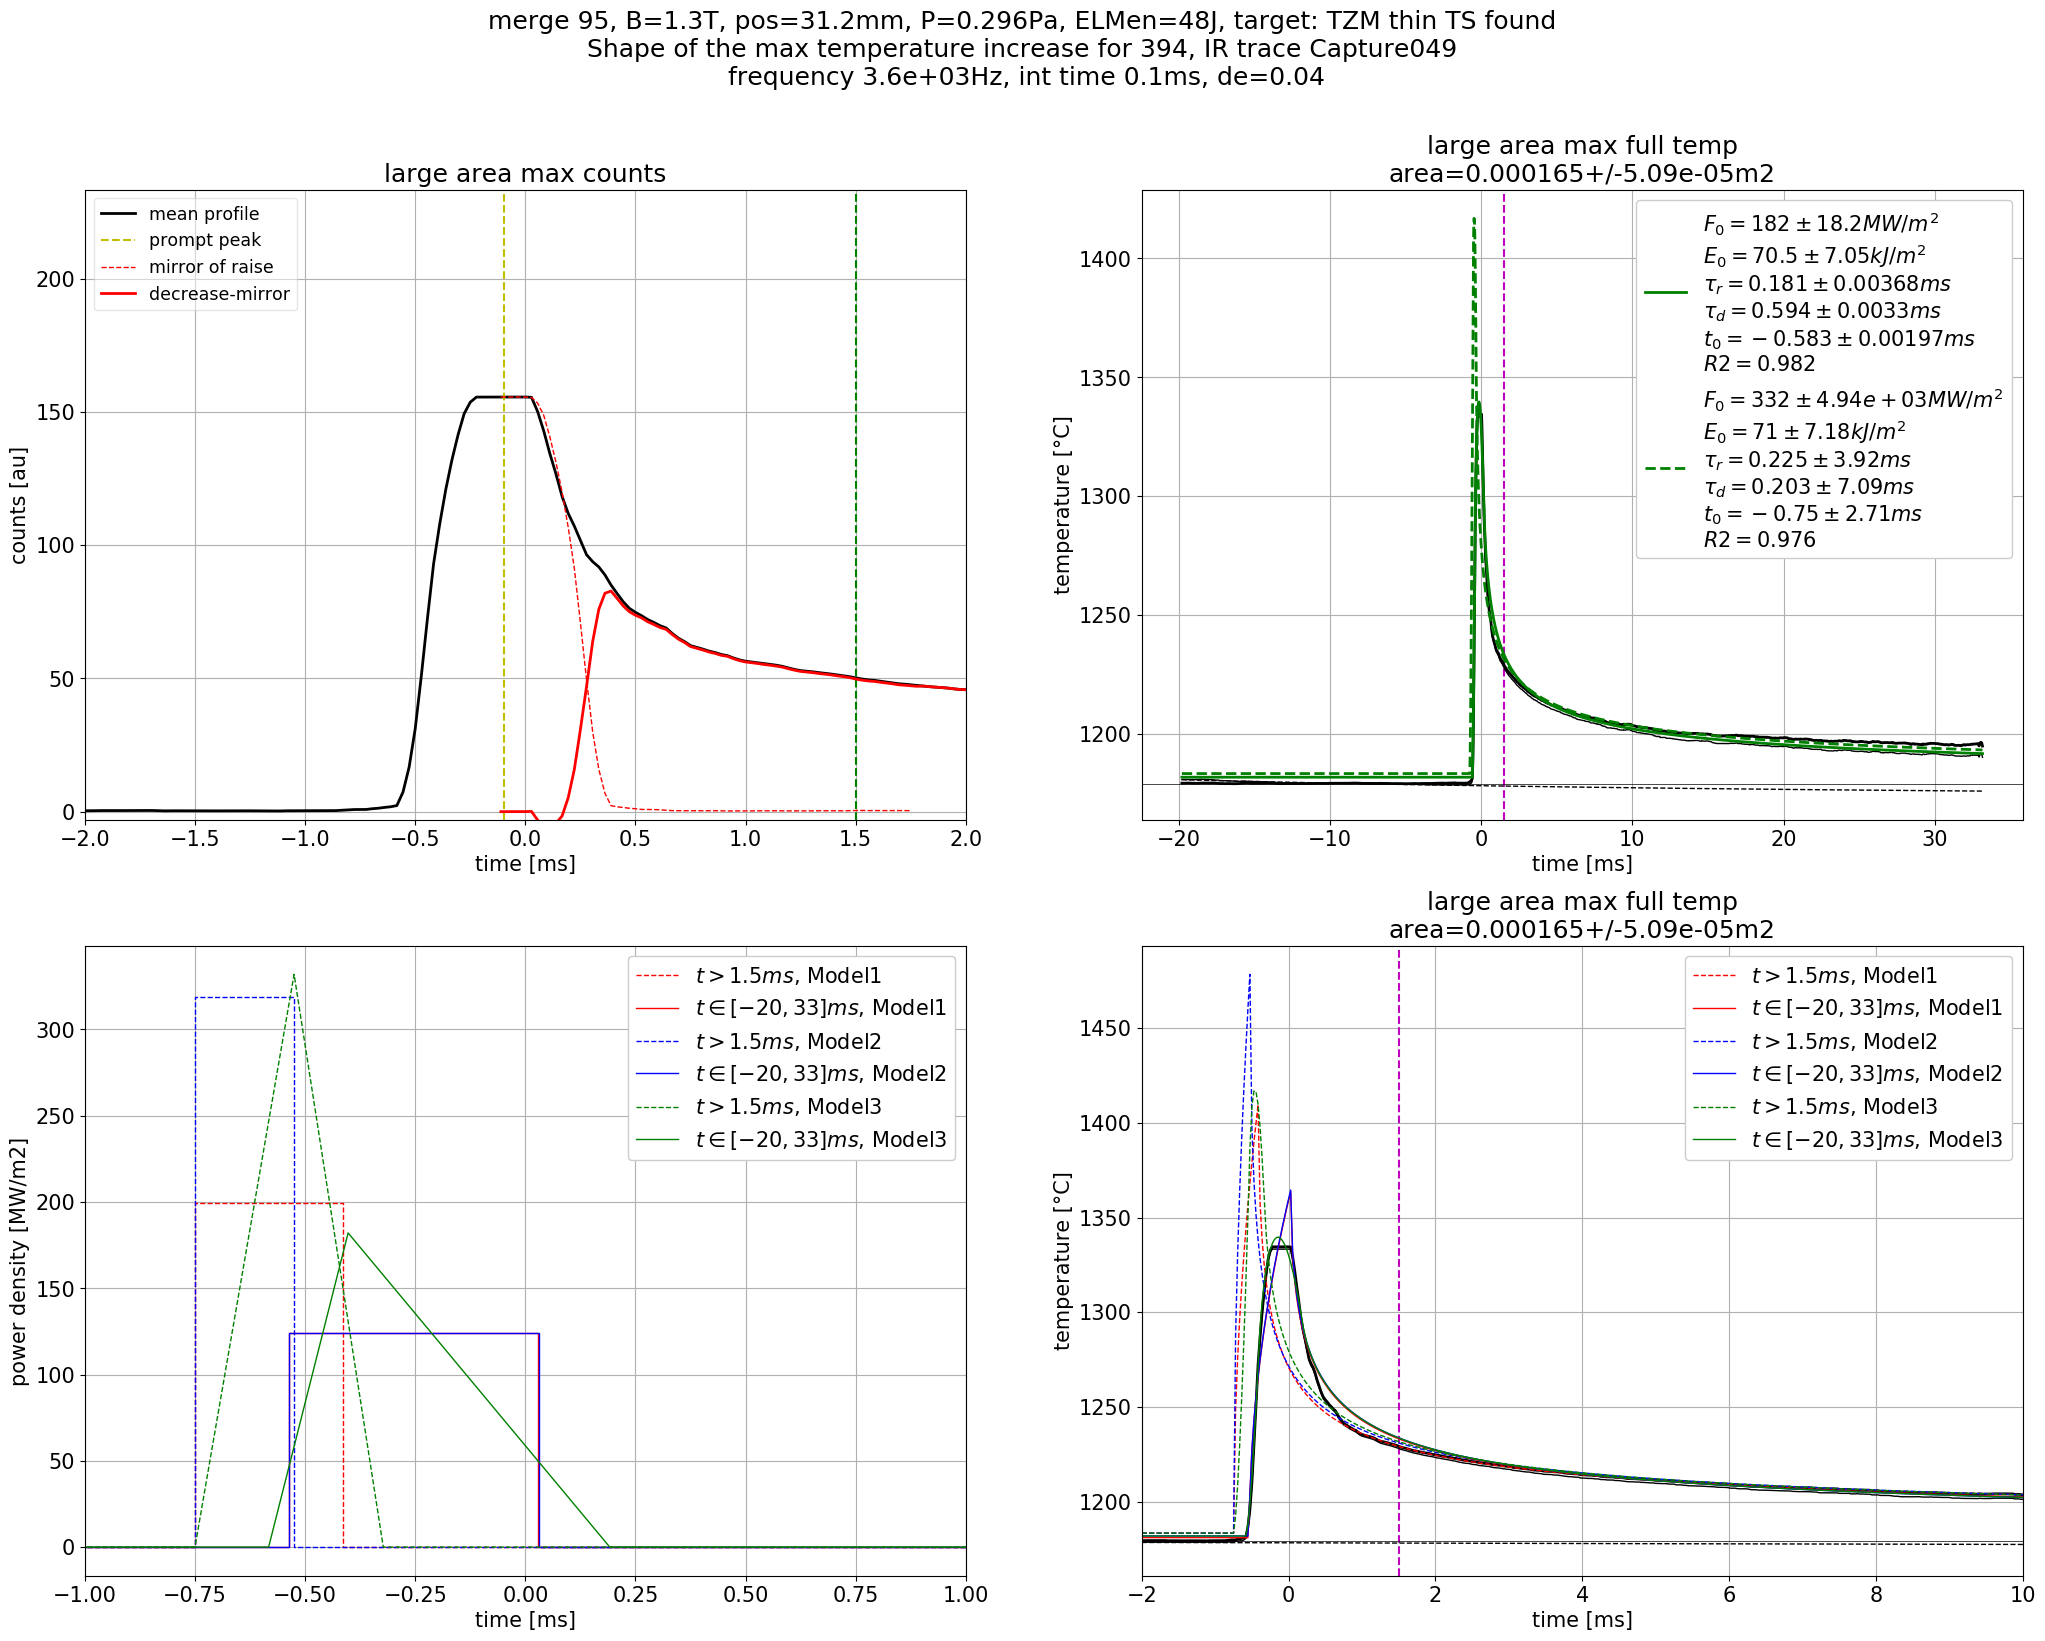
\includegraphics[width=0.7\linewidth,trim={750 550 10 115},clip]{Chapters/chapter3/figs/file_index_394_IR_trace_Capture049_43_old.png}
	\caption{Measured and fitted peak target temperature for a discharge in Stage 1 (ID 5 in \autoref{tab:table1}). In dashed green the fit of the temperature profile using the triangular Gaussian pulse model for t>1.5ms and in solid green the whole profile. The black dashed line indicates the cooling from the previous pulse and the thin solid black one is the peak target temperature not corrected for this.}
	\label{fig:IR4}
\end{figure}

\begin{figure}[!ht]
	\centering
	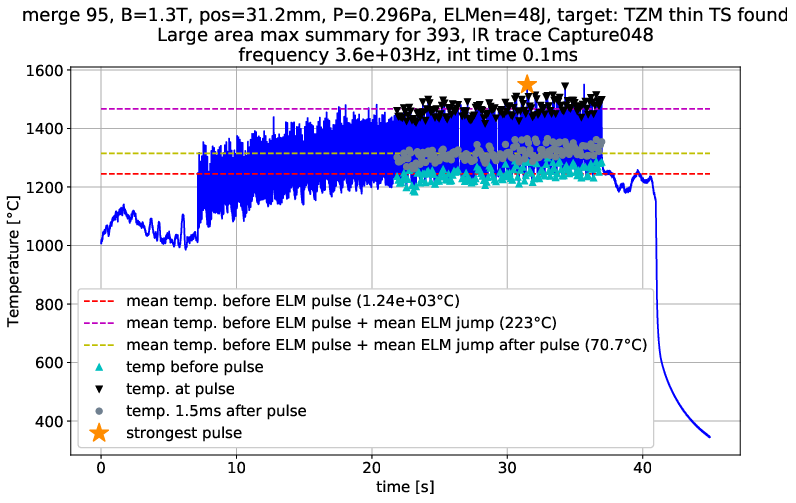
\includegraphics[width=0.7\linewidth,trim={5 5 55 65},clip]{Chapters/chapter3/figs/file_index_393_IR_trace_Capture048_46.png}
	\caption{Peak temperature of the target for low neutral pressure (ID 5 in \autoref{tab:table1}). To estimate the effect of the ELM-like pulse only the second half of the pulses is used, when the target is close to a steady state.}
	\label{fig:IR5}
\end{figure}

The result can be seen in the black dashed line in \autoref{fig:IR4} and in the increase of the peak temperature from the thin solid black line to the thick one. This correction is significant only for low neutral pressure conditions. In this cases it has to be taken also into account that it takes time to reach a thermal equilibrium after the ELM-like pulse train is started. To minimize this slow variation only the second 150 of the ELM-like pulses within a 300 strong scan is used to construct the average profile as it can be seen from \autoref{fig:IR5}.

\begin{figure}[!ht]
    % \hspace*{+10mm}
     \centering
     \begin{subfigure}{0.7\linewidth}
         \centering
        \hspace*{-5mm}
         %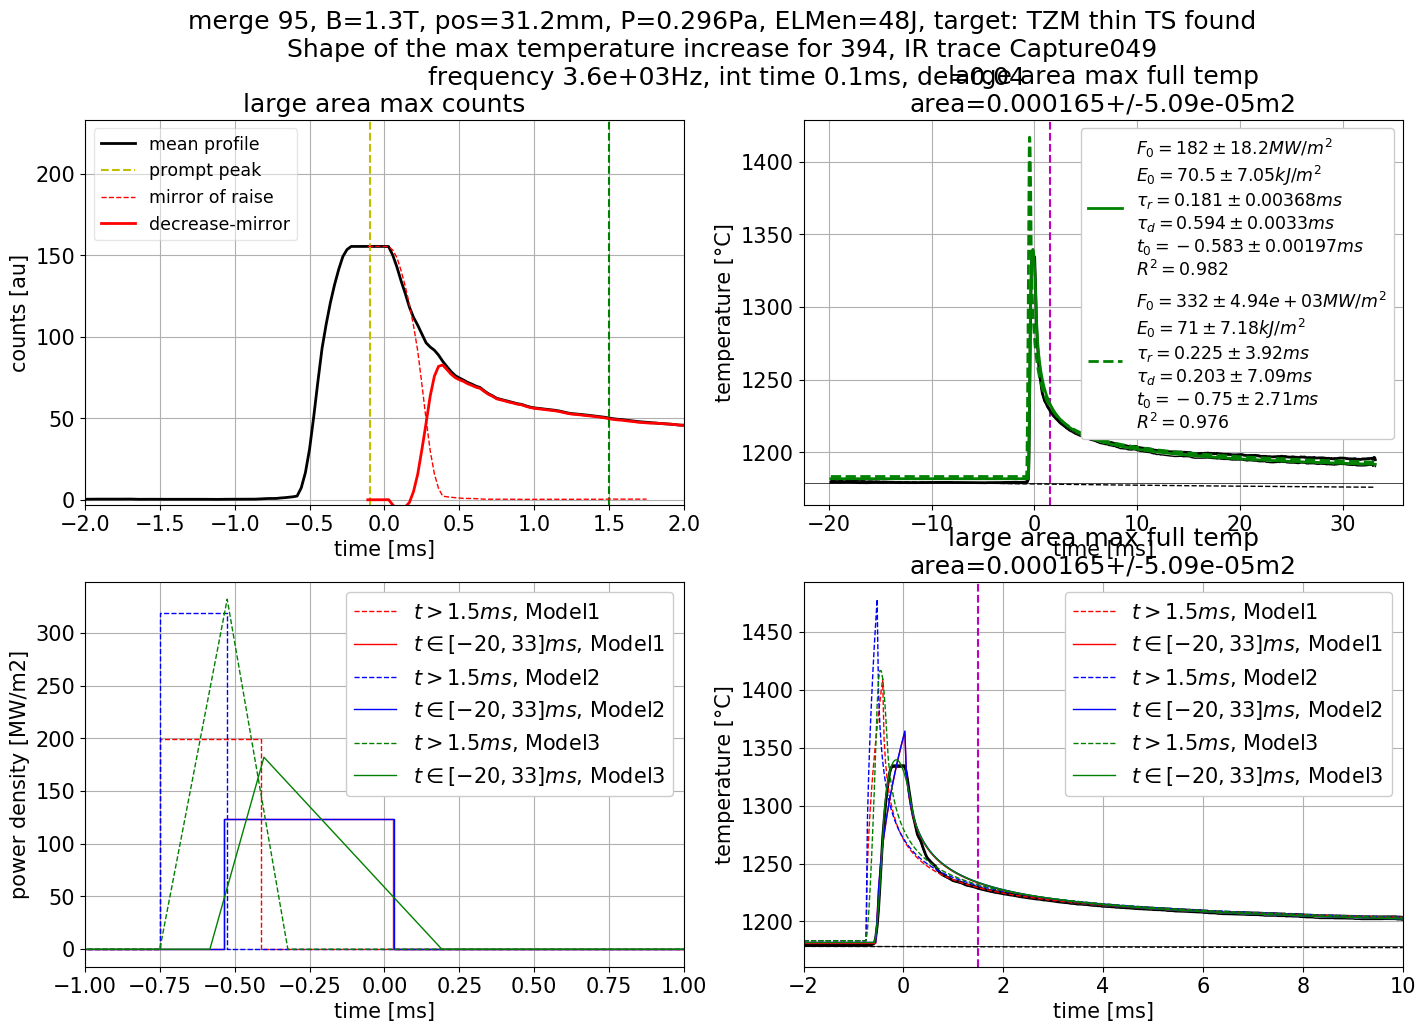
\includegraphics[width=\textwidth,trim={750 10 0 680},clip]{Chapters/chapter3/figs/file_index_394_IR_trace_Capture049_43.png}
         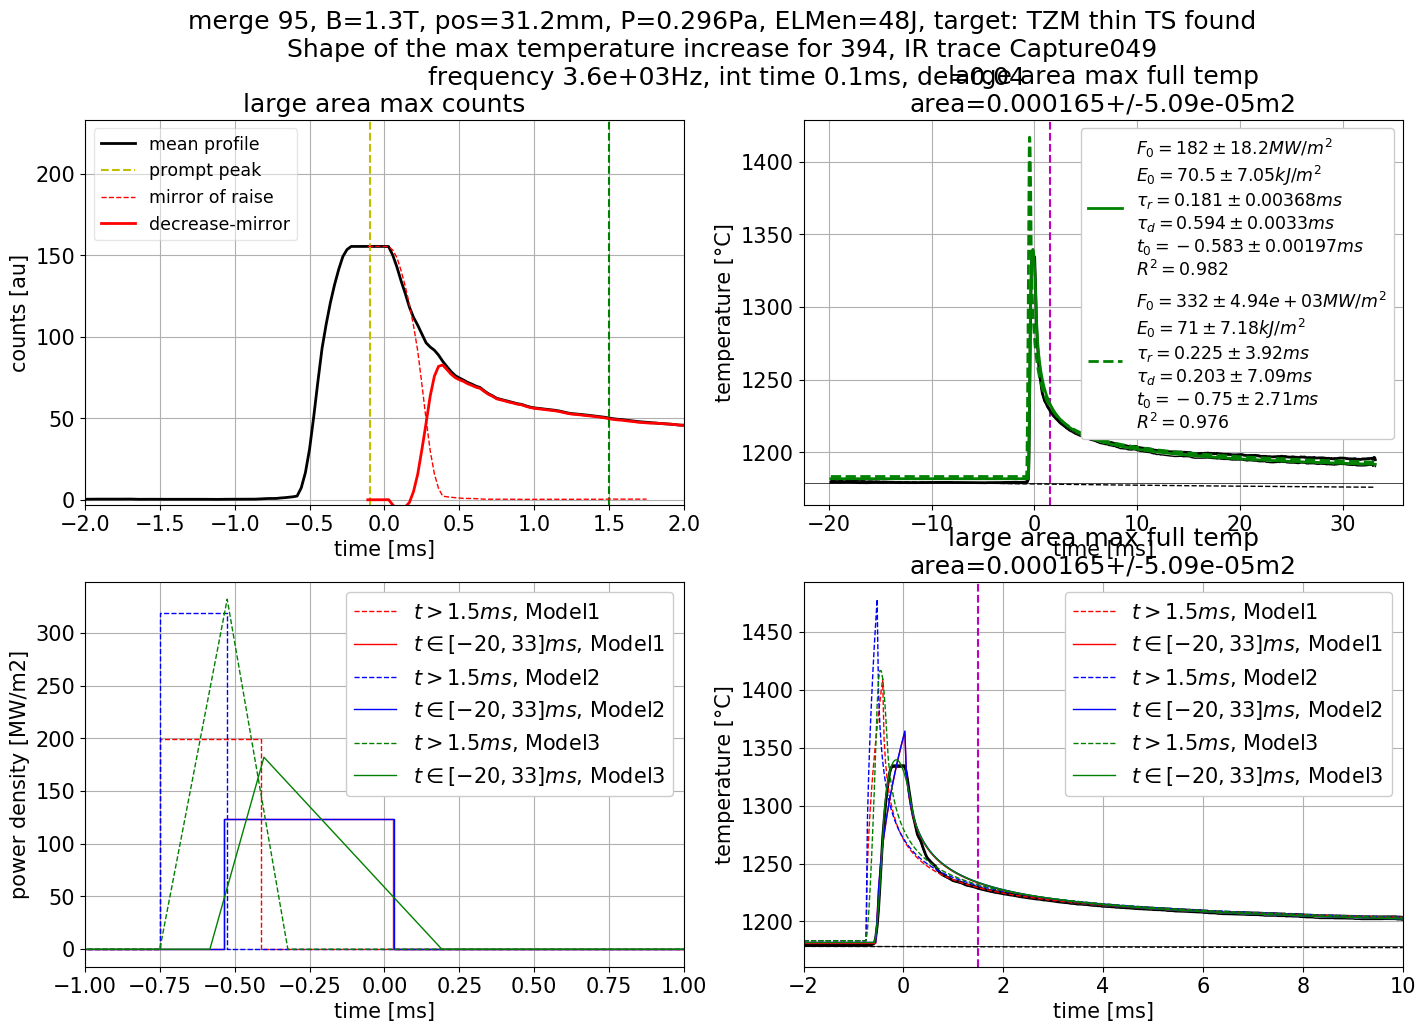
\includegraphics[width=0.8\textwidth,trim={510 5 5 415},clip]{Chapters/chapter3/figs/file_index_394_IR_trace_Capture049_43.png}
         % \vspace*{-30mm}
         \caption{\phantom{ww}}
         \label{fig:IR6a}
         %{\color{white}\caption{\phantom{wew}}\label{fig:TSa}}
     \end{subfigure}
     \hfill
    % \vspace*{+22mm}
    \begin{subfigure}{0.7\linewidth}
         \centering
         %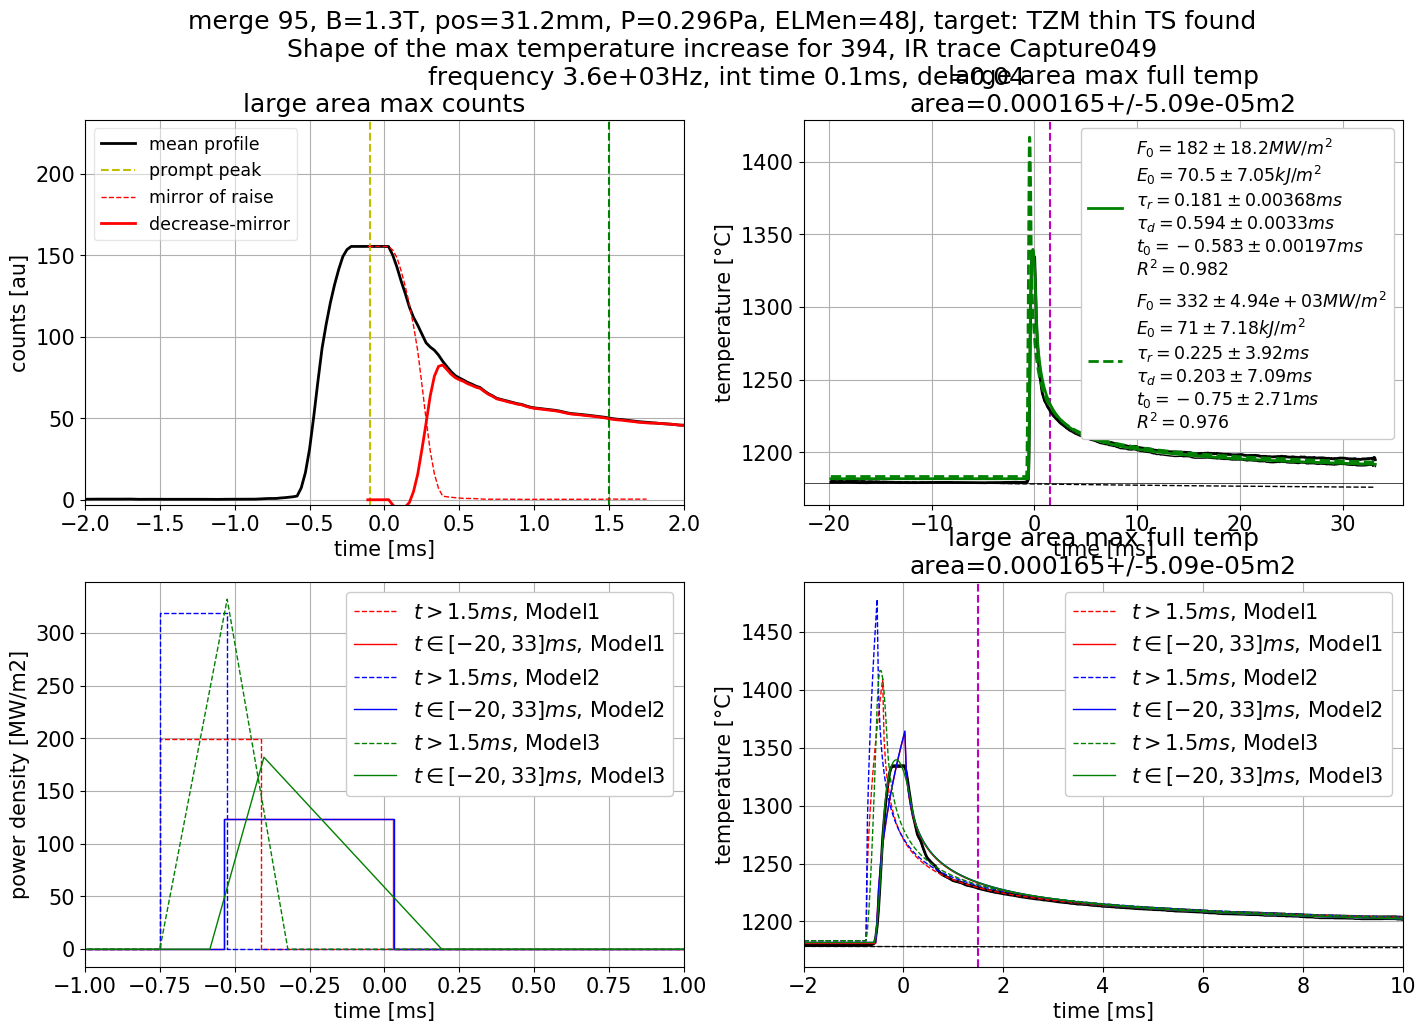
\includegraphics[width=\textwidth,trim={5 10 770 680},clip]{Chapters/chapter3/figs/file_index_394_IR_trace_Capture049_43.png}
         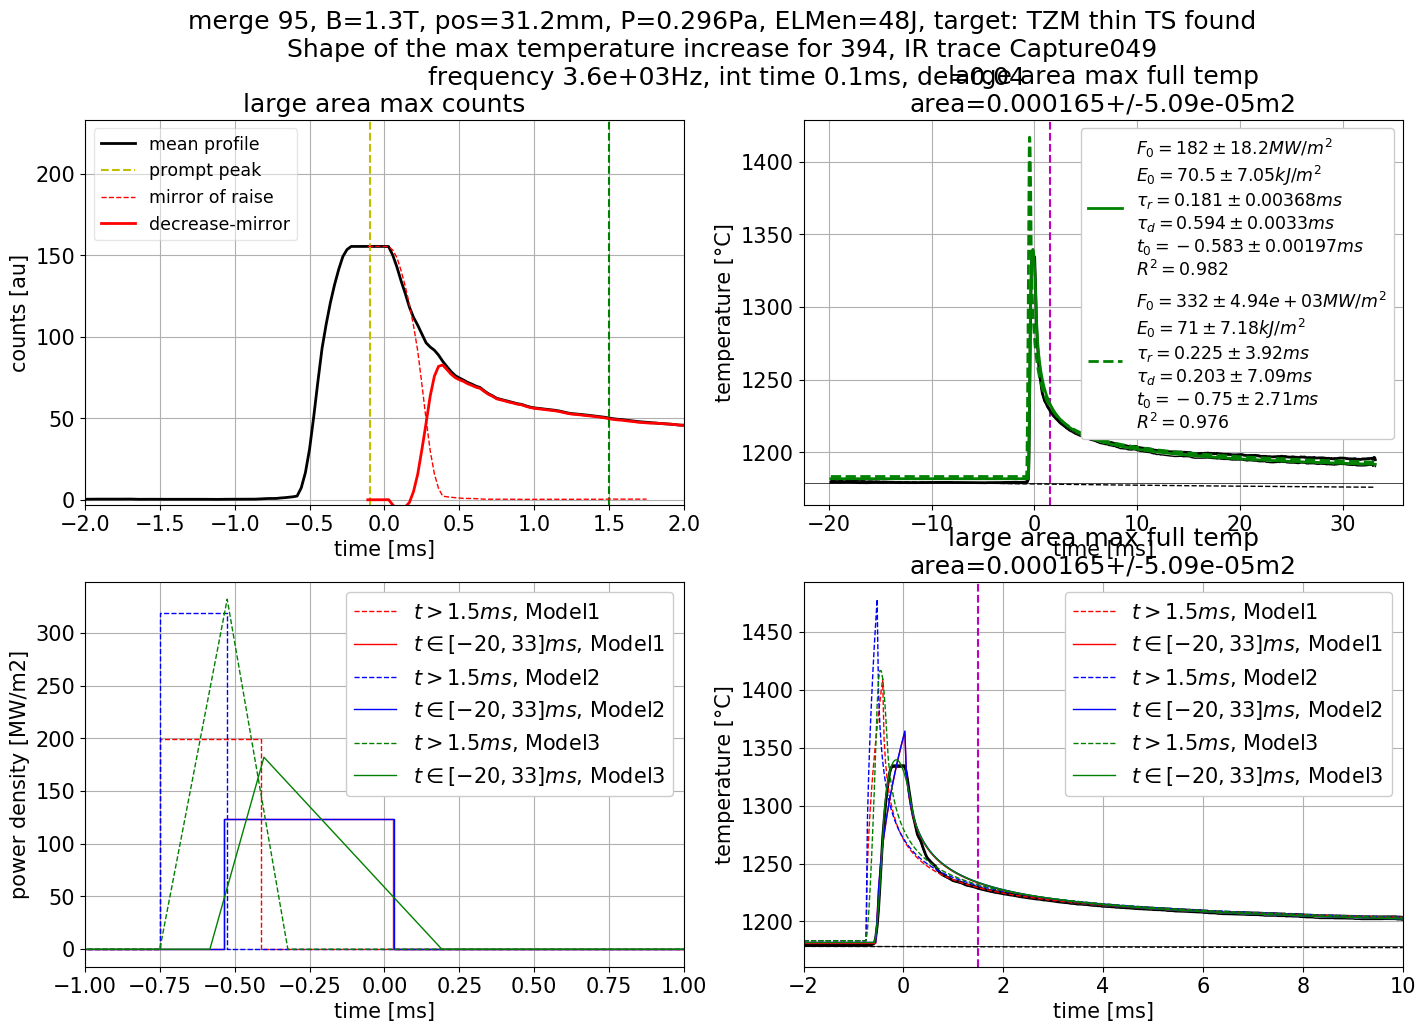
\includegraphics[width=0.8\textwidth,trim={5 5 515 415},clip]{Chapters/chapter3/figs/file_index_394_IR_trace_Capture049_43.png}
         % \vspace*{-30mm}
         \caption{\phantom{wew}}
         \label{fig:IR6b}
         %{\color{white}\caption{\phantom{wew}}\label{fig:TSb}}
     \end{subfigure}
        % \vspace*{+20mm}
        \caption{Comparison of the peak power density profiles (\subref{fig:IR6b}) result of fitting the peak temperature curve (\subref{fig:IR6a}) the with different analytical solutions for the lowest available neutral pressure conditions (ID 5 in \autoref{tab:table1}). All find adequate values for the energy density even with radically different peak durations. Dashed lines are obtained fitting from 1.5 to 30ms while solid ones from -20 to 30ms. In magenta 1.5ms after the temperature peak.}
        \label{fig:IR6}
\end{figure}

Considering all this a fit of the ELM-like pulse with the lowest neutral pressure can be used to compare the performance of the different models. As shown in \autoref{fig:IR6} all models fit well the slowly decreasing peak temperature slope and return a power density within 10\% of each other. Model3 fits best also the peak when the entire time axis is used.

\begin{figure}[!ht]
    % \hspace*{+10mm}
     \centering
     \begin{subfigure}{0.7\linewidth}
         \centering
        \hspace*{-5mm}
         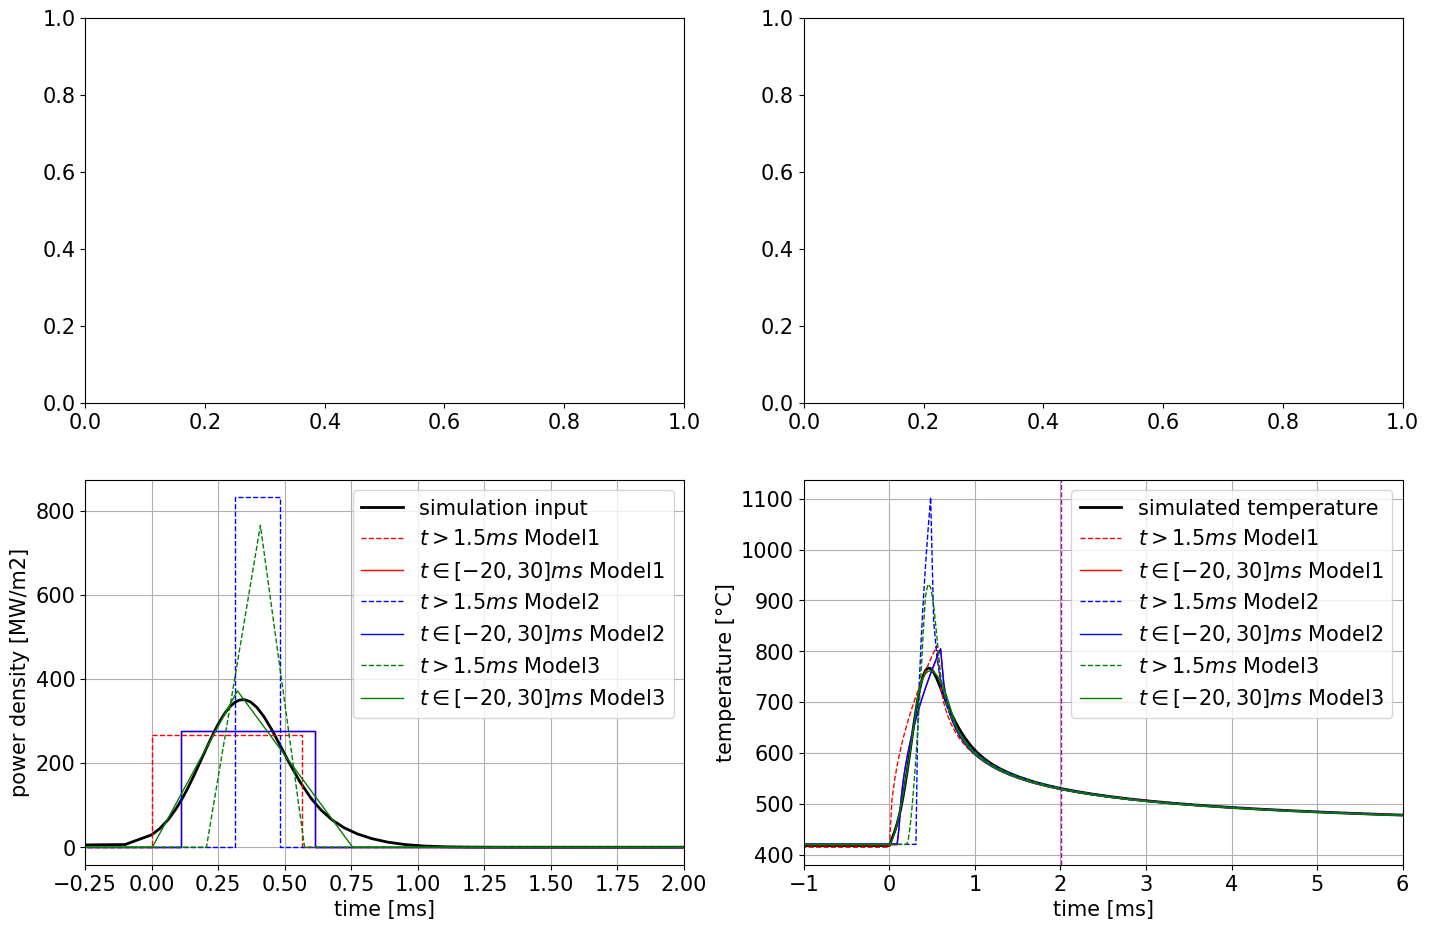
\includegraphics[width=0.8\textwidth,trim={510 5 5 330},clip]{Chapters/chapter3/figs/Figure_3.png}
         % \vspace*{-30mm}
         \caption{\phantom{wew}}
         \label{fig:IR7a}
         %{\color{white}\caption{\phantom{wew}}\label{fig:TSa}}
     \end{subfigure}
     \hfill
    % \vspace*{+22mm}
     \begin{subfigure}{0.7\linewidth}
         \centering
         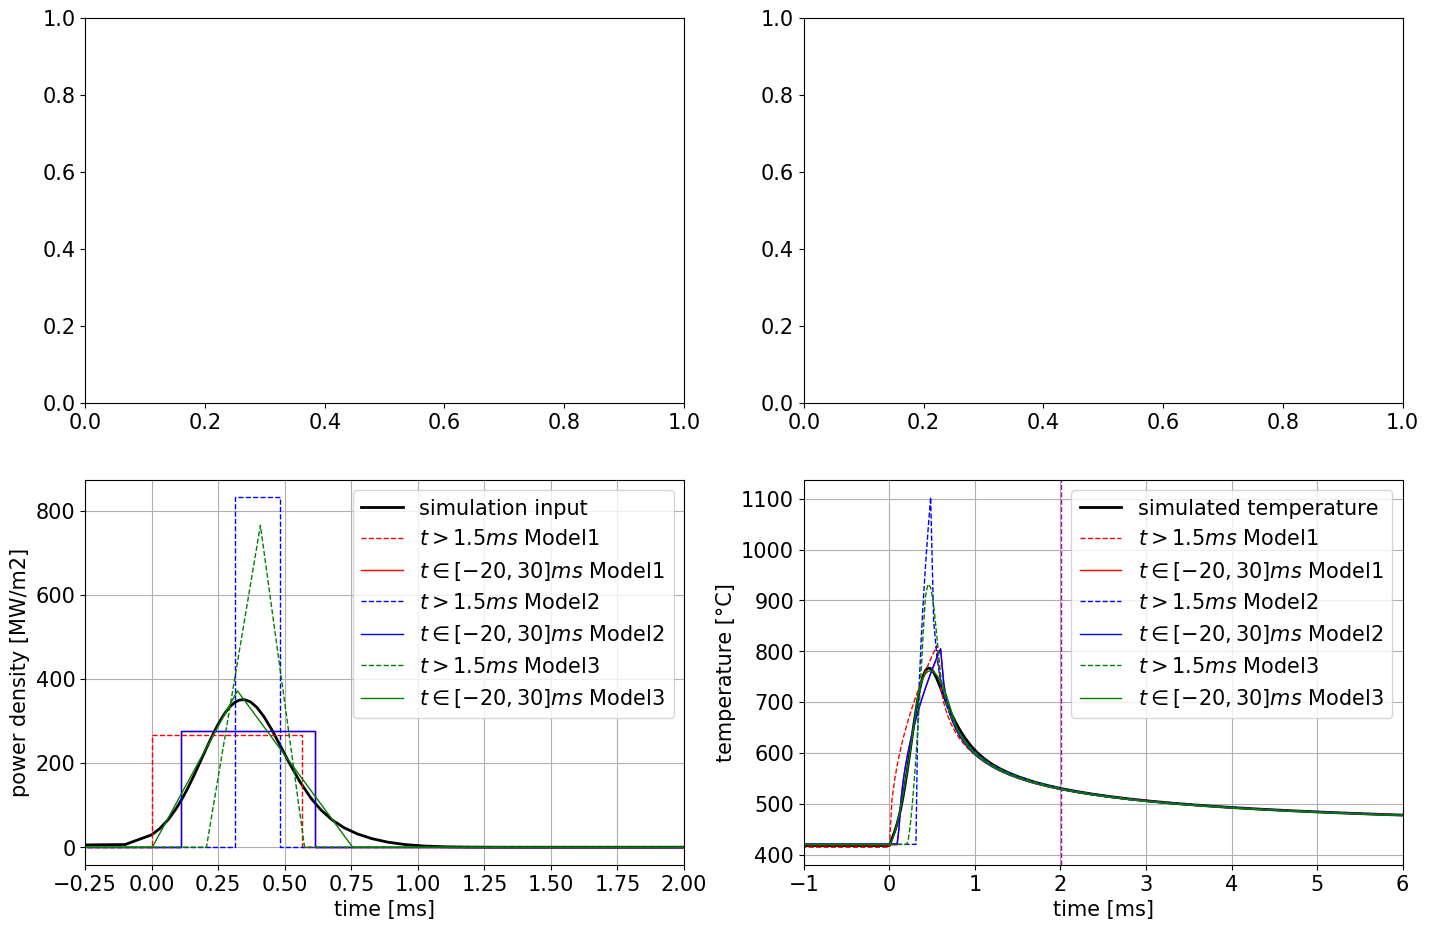
\includegraphics[width=0.8\textwidth,trim={5 5 515 330},clip]{Chapters/chapter3/figs/Figure_3.png}
         % \vspace*{-30mm}
         \caption{\phantom{wew}}
         \label{fig:IR7b}
         %{\color{white}\caption{\phantom{wew}}\label{fig:TSb}}
     \end{subfigure}
        % \vspace*{+20mm}
        \caption{Peak target temperature evolution (\subref{fig:IR7a}) calculated with the MSC.Marc/Mentat® code from a known heat flux profile made to be similar to the one caused by the CB in Magnum-PSI (\subref{fig:IR7b}) (solid black lines). That is fit with different analytical solutions and the inferred heat flux compared to the input. Dashed lines are obtained fitting from 1.5 to 30ms while solid ones the entire time axis. In magenta 1.5ms after the temperature peak.}
        \label{fig:IR7}
\end{figure}

The same comparison can be done with a simulated temperature rise obtained from a known input power profile. The MSC.Marc/Mentat® non linear FEM suite was used to reproduce a heat pulse similar to the one generated by the CB in terms of temporal and spatial variation and with temperature dependent material properties. The spatial distribution of the heat pulse was set as a Gaussian of radial extent consistent with what measured with TS ($1/e^2 \sim 1$cm) while the temporal variation was reproduced by fitting two Gaussians to the power profile from the plasma source. The comparison of the fits using the 3 models is shown in \autoref{fig:IR7}.

Model3 is capable of better reproducing the full temperature profile returning, for the full fit, with a power density shape very close to the input one. Even if the pulse duration when fitting only after 1.5ms is quite different from the input, the energy density is within 10\% of the input one for all cases and, as mentioned before, the uncertainty on the energy delivered to the target is $\sim$20\%, good enough for the purpose of this work.

\begin{figure}[!ht]
    \captionsetup{labelfont={color=black}}
    % \hspace*{+7mm}
     \centering
     \begin{subfigure}{0.6\linewidth}
         \centering
         % \vspace*{-0mm}
         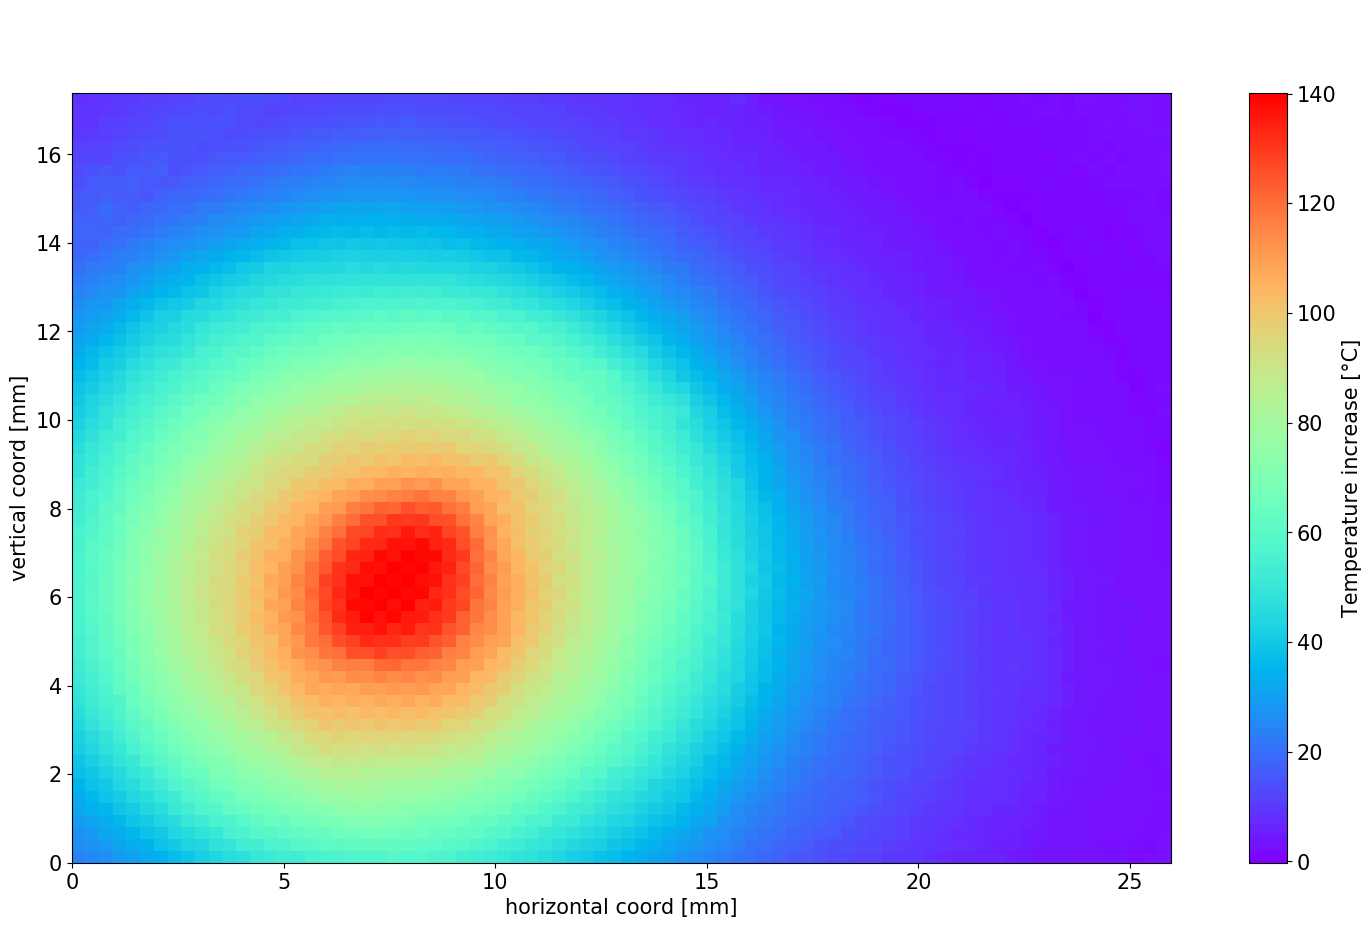
\includegraphics[width=\textwidth,trim={50 40 10 60},clip]{Chapters/chapter3/figs/file_index_393_IR_trace_Capture048_32b.png}
        \vspace*{-5mm}
        {\color{white}\caption{\phantom{wewew}}\label{fig:IR8a}}
     \end{subfigure}
     \hfill
    % \vspace*{+22mm}
     \begin{subfigure}{0.6\linewidth}
         \centering
         % \vspace*{-0mm}
         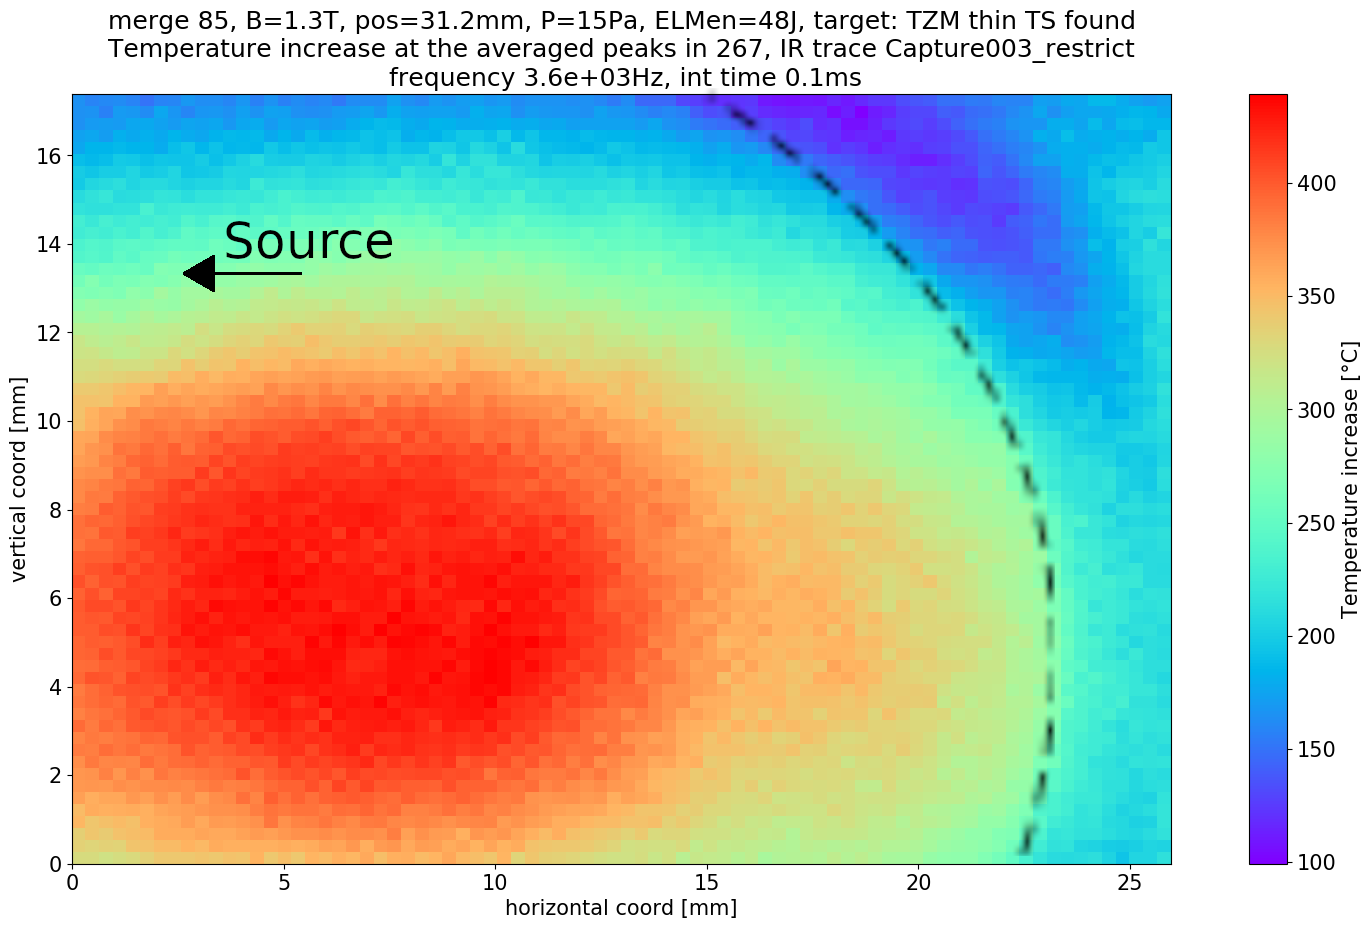
\includegraphics[width=\textwidth,trim={50 40 10 66},clip]{Chapters/chapter3/figs/file_index_267_IR_trace_Capture003_restrict_32b (copy).png}
        \vspace*{-5mm}
         {\color{white}\caption{\phantom{}}\label{fig:IR8b}}
     \end{subfigure}
        % \vspace*{+20mm}
        \caption{Peak temperature increase distribution over the steady state on the target. (\subref{fig:IR8a}) low neutral pressure conditions showing a clear confined peak (ID 5 in \autoref{tab:table1}). (\subref{fig:IR8b}) high neutral pressure case showing the temperature increase is not localized, possibly consistent with reflections of volumetric radiation or radiation of other origin (ID 10 in \autoref{tab:table1}). The black dashed line is the circular side of the cylindrical target. The arrow indicates where the source is outside the camera view.}
        \label{fig:IR8}
\end{figure}

To reinforce the argument on the origin of the prompt emission for high neutral pressure cases it is shown in \autoref{fig:IR8} the temperature profile at its peak for a low and high neutral pressure case. The low neutral pressure case (\subref{fig:IR8a}) shows a well defined peak with a radially symmetric decreasing profile. The high neutral pressure case (\subref{fig:IR8b}) is very different, with a much wider peak and a high temperature shadow from the peak to the edge of the target (marked in black). Note also the higher temperature outside the target itself. Considering the camera looks at the target at an angle and that the source is at the left of the field of view (see \autoref{fig:layout}), it is possible that the prompt peak could be due to radiation from the plasma itself reflected by the target. A definitive answer on what the origin of this radiation is cannot be given at this stage, but this observation further strengthen the case for only fitting the slowly decreasing temperature profile after the pulse.

\section{Details on the Bayesian calculations}\label{Details on the Bayesian calculations}

It will be detailed here how the expected properties of a plasma given a set of priors are calculated, compared with the measurements and used in the particle and power balance.

\subsection{Priors from B2.5 Eunomia}\label{Priors from B2.5 Eunomia}

In order to define the initial parameter space and the prior it is necessary to define the range and probability associated with all the axis of the parameter space.

For $T_e$ and $n_e$ the TS values are used and the range is defined as 6 times the uncertainty. The probability is calculated as a linear normal distribution with the uncertainty corresponding to 1 sigma.

The range and probabilities for $n_{H_2}/n_e$ are obtained from B2.5-Eunomia simulations for a steady state neutral pressure scan with 2 plasma source settings, ranging from attached to detached via increasing neutral hydrogen target chamber neutral pressure, carried out by Chandra.\cite{Chandra2021,Chandra2022} The simulations consider the whole plasma column source to target, but only data inside the target chamber and within 2cm of the axis are considered here (marked with $x$, versus other regions marked by a point in \autoref{fig:priors1}, \ref{fig:priors2}, \ref{fig:priors3}, \ref{fig:priors4}, \ref{fig:priors4b}, \ref{fig:priors5}).

\begin{figure}[!ht]
	\centering
	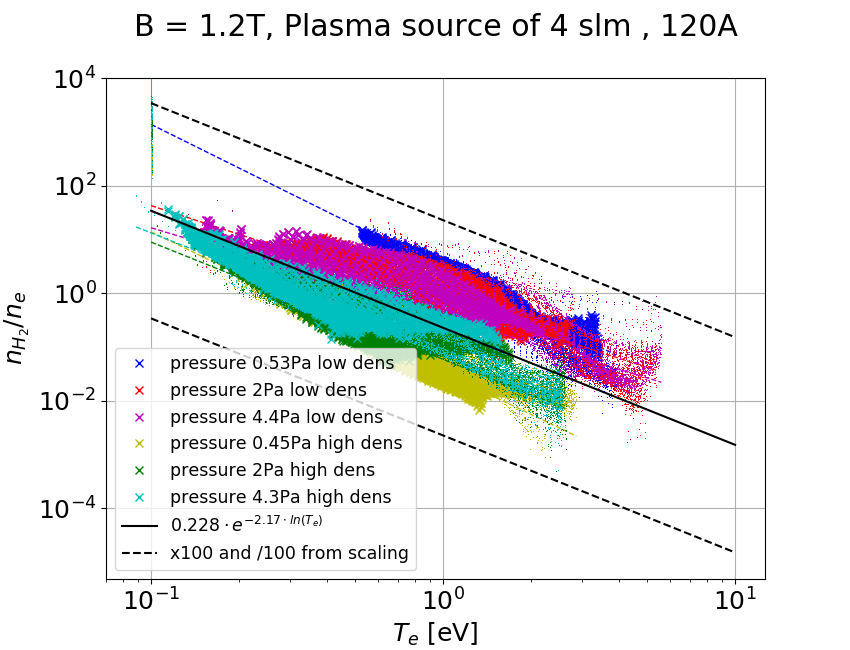
\includegraphics[width=0.7\linewidth,trim={0 0 30 45},clip]{Chapters/chapter3/figs/nH2_ne3.png}
	\caption{Correlation between molecular hydrogen and plasma density with temperature from B2.5-Eunomia modelling. The colored dashed lines are obtained with a linear log log fit for the single cases. The solid black line is obtained averaging the fitting parameters obtained.}
	\label{fig:priors1}
\end{figure}


As demonstrated by Den Harder\cite{DenHarder2015} the density decrease of $H_2$ in the plasma is mainly driven by rarefaction due to the high temperature of the plasma itself. For this reason a quite strong correlation between molecular hydrogen and plasma density ratio  and plasma temperature exists, shown in \autoref{fig:priors1}. The most likely ratio is obtained by fitting each simulation's results with a linear log log function and then averaging the fit parameters as shown in \autoref{fig:priors1}. The probability is defined as a normal distribution where 2 sigma corresponds to the black dashed lines, 100 and 1/100 times the fit value. The range is a significantly larger window around the dashed lines, to account for the large uncertainty coming from the fact that B2.5-Eunomia only simulates steady state conditions while the ELM-like burn through is a very dynamic one.

\begin{figure}[!ht]
	\centering
	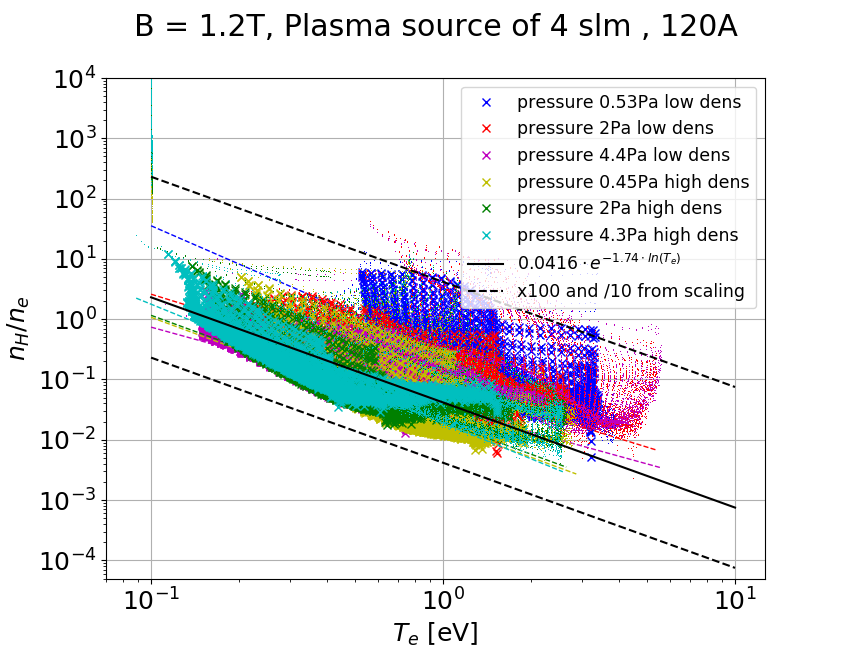
\includegraphics[width=0.7\linewidth,trim={0 0 30 45},clip]{Chapters/chapter3/figs/nH_ne3.png}
	\caption{Correlation between atomic hydrogen and plasma density with temperature from B2.5-Eunomia modeling. The colored dashed lines are obtained with a linear log log fit for the single cases. The solid black line is obtained averaging the fitting parameters obtained.}
	\label{fig:priors2}
\end{figure}

The simulations are used to provide also range and probability for $n_H/n_e$. Atomic hydrogen is generated from recombination and from $H_2$ interaction with plasma and various molecules, so its density is only weakly correlated with plasma temperature and density, as shown in \autoref{fig:priors2}. 
The probability was calculated with a linear normal distribution with nominal value from the fit (calculated in the same fashion as for $n_{H_2}/n_e$) and 2 sigma arbitrarily assigned as per the dashed line in \autoref{fig:priors2}.
% no, this was reversed Given the large range and spread in $n_H/n_e$, the use of the probability for $n_H/n_e$ was later dropped and instead a linear uniform probability for all values was used.

\begin{figure}[!ht]
	\centering
	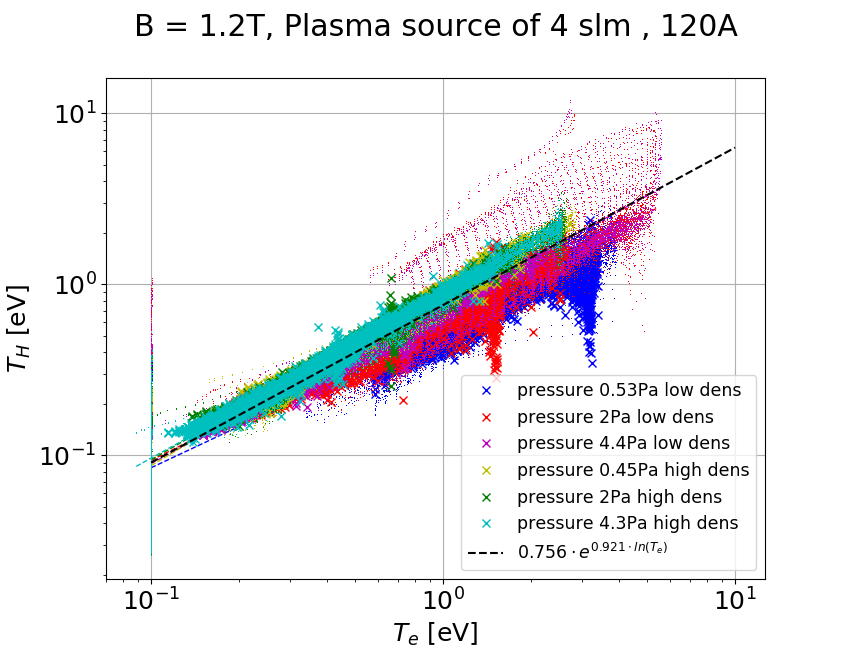
\includegraphics[width=0.7\linewidth,trim={0 0 30 45},clip]{Chapters/chapter3/figs/TH_Te3.png}
	\caption{Correlation between atomic hydrogen and electron temperature from B2.5-Eunomia modeling}
	\label{fig:priors3}
\end{figure}

\begin{figure}[!ht]
	\centering
	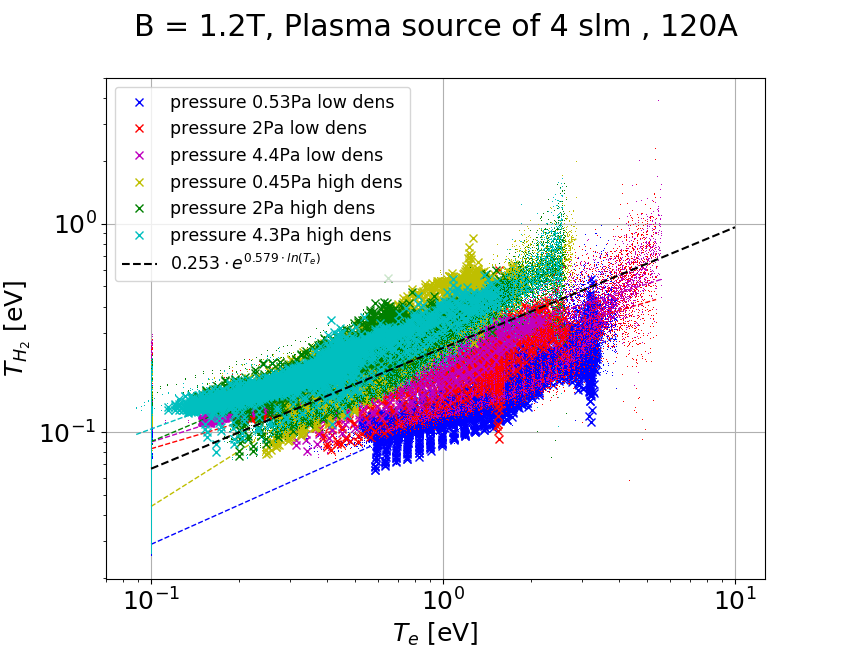
\includegraphics[width=0.7\linewidth,trim={0 0 30 45},clip]{Chapters/chapter3/figs/TH2_Te3.png}
	\caption{Correlation between $H_2$ and electron temperature from B2.5-Eunomia modelling. The colored dashed lines are obtained with a linear log log fit for the single cases. The solid black line is obtained averaging the fitting parameters obtained. This is assumed to be the same as ${H_2}^+$ temperature, while to obtain $H^-$ temperature 2.2eV are added to account for the $H_2$ dissociation energy.}
	\label{fig:priors4}
\end{figure}

\begin{figure}[!ht]
	\centering
	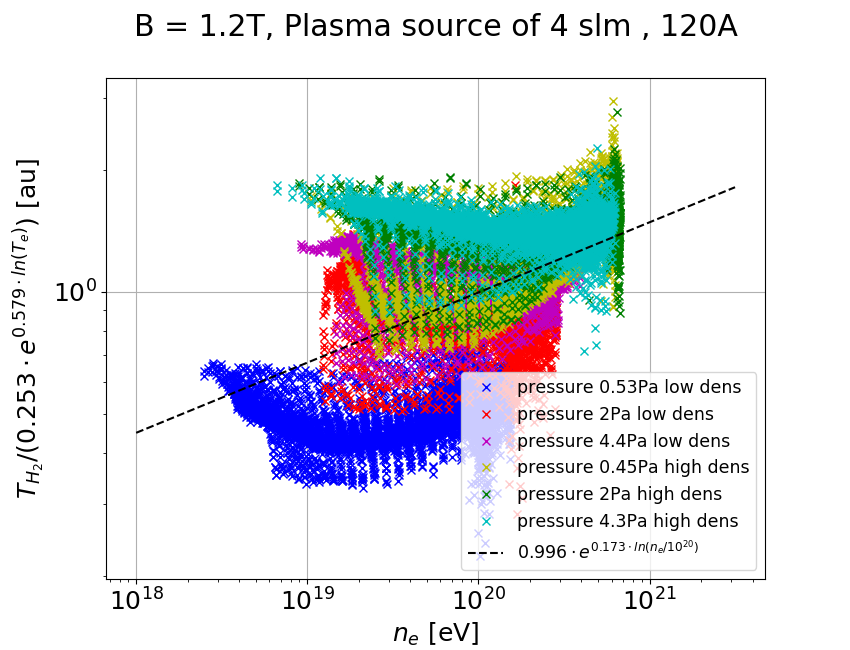
\includegraphics[width=0.7\linewidth,trim={0 0 30 45},clip]{Chapters/chapter3/figs/TH2_Te_ne3.png}
	\caption{Residuals from fitting $T_{H_2}$ with the scaling from \autoref{fig:priors4} and their weak dependence on the plasma density. The linear log log scaling in black is obtained by fitting all points at once.}
	\label{fig:priors4b}
\end{figure}

\begin{figure}[!ht]
	\centering
	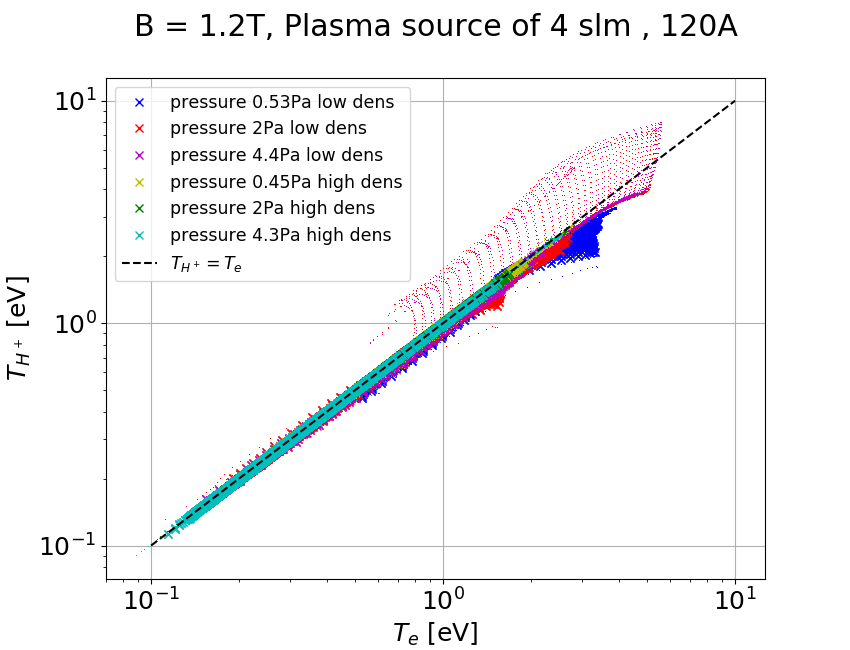
\includegraphics[width=0.7\linewidth,trim={0 0 30 45},clip]{Chapters/chapter3/figs/THp_Te3.png}
	\caption{Correlation between $H^+$ and electron temperature from B2.5-Eunomia modelling. The dashed line indicates $T_{H^+}=T_e$.}
	\label{fig:priors5}
\end{figure}

Other quantities that are part of the plasma state and had to be determined to calculate reaction rates and other coefficients are the temperatures of all species. To reduce the number of variables in the Bayesian algorithm their uncertainty is in this work not considered and only the nominal values are used. The correlations are shown in \autoref{fig:priors3}, \ref{fig:priors4}, \ref{fig:priors5} for $H$, $H_2$ and $H^+$ temperature respectively where the black dashed lines indicates the values used. For $T_H$ and $T_{H_2}$ the fit is obtained in the same fashion as $n_H/n_e$ while for $T_{H^+}$ it is assumed $T_{H^+}=T_e=T_{plasma}$. For $T_{H_2}$ in particular a weak dependence on the plasma density is present, whose estimate is shown in \autoref{fig:priors4b} and can be due to an increase of the collisionality for higher density and a better coupling with the neutrals, resulting in a correction factor to apply to the dependency on $T_e$ alone. Given ${H_2}^+$ is mostly originated from $H_2$ it is considered $T_{H_2}=T_{{H_2}^+}$. This is valid for $H^-$ too, but because it can get some of the $H_2$ binding energy (2.2eV per atom) 2.2eV are added to $T_{H_2}$ to estimate $T_{H^-}$.\cite{Verhaegh2020}


\subsection{Priors from AMJUEL}\label{Priors from AMJUEL}
Ionised hydrogen molecules are generated mainly from $H_2$ so their density prior is calculated with AMJUEL\cite{Reiter2017}, a library that, among others, contains $n_{H^-}/n_{H_2}$ and $n_{{H_2}^+}/n_{H_2}$ density ratios in an equilibrium plasma for given plasma temperature and density (Section 12.58, 12.59, 11.11, 11.12). The conditions of an ELM-like pulse can potentially deviate significantly from equilibrium, so a wide range around equilibrium is considered as prior and a linear uniform distribution as likelihood.


\subsection{Priors range optimization}\label{Priors range optimization}
In order to optimize the $n_{H}/n_e$ range to only useful values a combination of the information from \autoref{fig:priors1} and the OES measurement is used. For each $T_e$ / $n_e$ combination it is calculated what is the emission from EIR via the ADAS PEC coefficients and subtracted from the OES measurement. It is then calculated what is the $n_{H}/n_e$ required to recreate via EIE each residual line emission plus its uncertainty. The largest $n_{H}/n_e$, limited by a predefined multiplier times the value from the B2.5-Eunomia fit, will be the highest value considered for that particular $T_e$ / $n_e$ combination. The lower limit will be taken as a small fraction of the maximum value, again limited by a predefined multiplier times the value from the B2.5-Eunomia fit. In this way parts of the range of $n_{H}/n_e$ that would cause an excessive line emission are automatically excluded and the prior range is assigned efficiently.

The same process is applied to the $n_{H_2}/n_e$ prior. For each $T_e$ / $n_e$ / $n_{H}/n_e$ the total emission from EIR and EIE is subtracted from the OES measurement and the $n_{H_2}/n_e$ required to match the residual is calculated with the Yacora coefficients for the $H_2$ dissociation reaction. For the $n_{{H_2}^+}/n_{H_2}$ prior the emission from EIR, EIE, $H_2$ dissociation is considered. Consequently for the $n_{{H}^-}/n_{H_2}$ prior also the emission from ${H_2}^+$ is considered.

\subsection{Emissivity}\label{Emissivity}

The emissivity is calculated for known precursors densities via the ADAS PECs and Yacora population coefficients.\cite{Verhaegh2020}
The Photon Emission Coefficients (PEC, photons $m^3/s$) coefficients are defined as the number of photons generated per second per unit of the precursors density. The number of photons for the transition $p \rightarrow q$ is equal to the product of density of the excited state $p$ and the Einstein coefficient $A_{pq}$ so the emission generated by atomic excitation and recombination can be expressed as per \autoref{eq:emiss1} and \ref{eq:emiss2}, where it is also highlighted what is intended as population coefficient ($PC_i$).

\begin{equation}
\label{eq:emiss1}
\begin{aligned}
\epsilon^{exc}_{pq} = PEC^{exc}_{pq}(T_e,n_e) n_e n_{H} = A_{pq} \underbrace{ \frac{n_{H(p)}}{n_e n_{H}}}_{PC_{exc}} n_e n_{H} 
\end{aligned}
\end{equation}

\begin{equation}
\label{eq:emiss2}
\begin{aligned}
\epsilon^{rec}_{pq} = PEC^{rec}_{pq}(T_e,n_e) n_e n_{H^+{}} = A_{pq} \underbrace{\frac{n_{H(p)}}{n_e n_{H^+{}}}}_{PC_{rec}} n_e n_{H^+{}}
\end{aligned}
\end{equation}

The line emission due to molecular reactions is similarly calculated via the Yacora population coefficients as per \autoref{eq:emiss3}, \ref{eq:emiss4}, \ref{eq:emiss5} and \ref{eq:emiss6}. It is also shown which reaction was considered in building the coefficients, and the variables necessary to calculate the coefficients. As mentioned $T_H$, $T_{H_2}$ are determined from the B2.5-Eunomia simulation while $T_{H_2} \approx T_{{H_2}^+} \approx T_{H^-}-2.2eV$.

\begin{equation}
\label{eq:emiss3}
\begin{aligned}
\epsilon^{{H_2}^+{}}_{pq} =& A_{pq} PC_{{H_2}^+{}}(T_e,n_e) n_e n_{{H_2}^+{}} \\
reactions:\ &{H_2}^+{} + e^-{} \rightarrow H(p) + H^+{} + e^-{} \\ 
\ &{H_2}^+{} + e^-{} \rightarrow H(p) + H(0)
\end{aligned}
\end{equation}

\begin{equation}
\label{eq:emiss4}
\begin{aligned}
\epsilon^{{H_2}}_{pq} =& A_{pq} PC_{{H_2}}(T_e,n_e) n_e n_{{H_2}} \\
reaction:\ &{H_2}^+{} + e^-{} \rightarrow H(p) + H(1) + e^-{}
\end{aligned}
\end{equation}

\begin{equation}
\label{eq:emiss5}
\begin{aligned}
\epsilon^{{H}^-{}+{H_2}^+{}}_{pq} =& A_{pq} PC_{{H}^-{}+{H_2}^+{}}(T_e,T_{{H_2}^+{}},T_{{H}^-{}},n_e) n_{{H_2}^+{}} n_{{H}^-{}} \\
reaction:\ &{H}^-{}+{H_2}^+{} \rightarrow H(p) + H_2
\end{aligned}
\end{equation}

\begin{equation}
\label{eq:emiss6}
\begin{aligned}
\epsilon^{{H}^-{}+{H}^+{}}_{pq} =& A_{pq} PC_{{H}^-{}+{H}^+{}}(T_e,T_{{H}^+{}},T_{{H}^-{}},n_e) n_{{H}^+{}} n_{{H}^-{}} \\
reaction:\ &{H}^-{}+{H}^+{} \rightarrow H(p) + H(1)
\end{aligned}
\end{equation}

The total calculated emissivity and its uncertainty are determined as per \autoref{eq:emiss7} with $\sigma_{ADAS}$ and $\sigma_{Yacora}$ the uncertainty on the coefficients mentioned before.

\begin{equation}
\label{eq:emiss7}
\begin{aligned}
\epsilon^{calc}_{pq} =& \epsilon^{exc}_{pq} + \epsilon^{rec}_{pq} + \epsilon^{{H_2}^+{}}_{pq} + \epsilon^{{H_2}}_{pq} + \epsilon^{{H}^-{}+{H_2}^+{}}_{pq} + \epsilon^{{H}^-{}+{H}^+{}}_{pq}
\\
\sigma^{calc}_{\epsilon_{pq}} =& \left\{ {\sigma_{ADAS}}^2 \left({\epsilon^{exc}_{pq}}^2 + {\epsilon^{rec}_{pq}}^2\right) + \right. \\ &\left. + {\sigma_{Yacora}}^2 \left({\epsilon^{{H_2}^+{}}_{pq}}^2 + {\epsilon^{{H_2}}_{pq}}^2 + {\epsilon^{{H}^-{}+{H_2}^+{}}_{pq}}^2 + {\epsilon^{{H}^-{}+{H}^+{}}_{pq}}^2\right) \right\}^{1/2}
\end{aligned}
\end{equation}

The line emissivity measurement is compared with the expectation. For each precursor combination and line is calculated what is the likelihood that $y_{pq}=0$ with \autoref{eq:emiss8a}
\begin{equation}
\label{eq:emiss8a}
\begin{aligned}
y_{pq} = \epsilon^{calc}_{pq}-\epsilon^{measure}_{pq} ,& \sigma_{y_{pq}} = \sqrt{{\sigma_{\epsilon_{pq}}^{calc}}^2 + {\sigma_{\epsilon_{pq}}^{measure}}^2}
\\
L(y_{pq} = 0|\Theta) =& \frac{1}{\sigma_{y_{pq}} \sqrt{2\pi}} e^{-\frac{1}{2} \left( \frac{y_{pq}}{\sigma_{y_{pq}}} \right)^2 }
\end{aligned}
\end{equation}
where $\Theta$ represent the specific combination of precursors that lead to the emission $\epsilon^{calc}_{pq}$.

Following Bayes theorem the posterior (probability of the combination of precursors generating the measurements) is calculated as the likelihood of the measurement being generated by the precursors times the probability associated with the precursors themselves divided by the probability of the measured data. For the case in which only one emission line is included in the model this is expressed in \autoref{eq:emiss8b}

\begin{equation}
\label{eq:emiss8b}
\begin{aligned}
P(\Theta|y_{pq} = 0) = \frac{L(y_{pq} = 0|\Theta) P(\Theta)}{P(y_{pq} = 0)}
\end{aligned}
\end{equation}

Where $P(y_{pq} = 0)$ acts as a normalisation factor. The final product of all probabilities will be anyway normalised, so this term can be neglected. $P(\Theta)$ is  the product of the probability associated with every combination of precursors (see \autoref{Priors from B2.5 Eunomia}, \ref{Priors from AMJUEL} and \ref{Prior probability distribution}). The probability of fitting all the lines $P_{\epsilon}$ is then determined with \autoref{eq:emiss8}.

\begin{equation}
\label{eq:emiss8}
\begin{aligned}
P_{\epsilon} =& P(\Theta) \prod_{p=4,q=2}^{p=8} P(\Theta|y_{pq} = 0)
\end{aligned}
\end{equation}

For this calculations $\sigma_{ADAS}$ and $\sigma_{Yacora}$ were assumed 10\% and 20\% respectively.

\subsection{Balance over the plasma column}\label{Balance over the plasma column}

\begin{figure*}
	\centering
	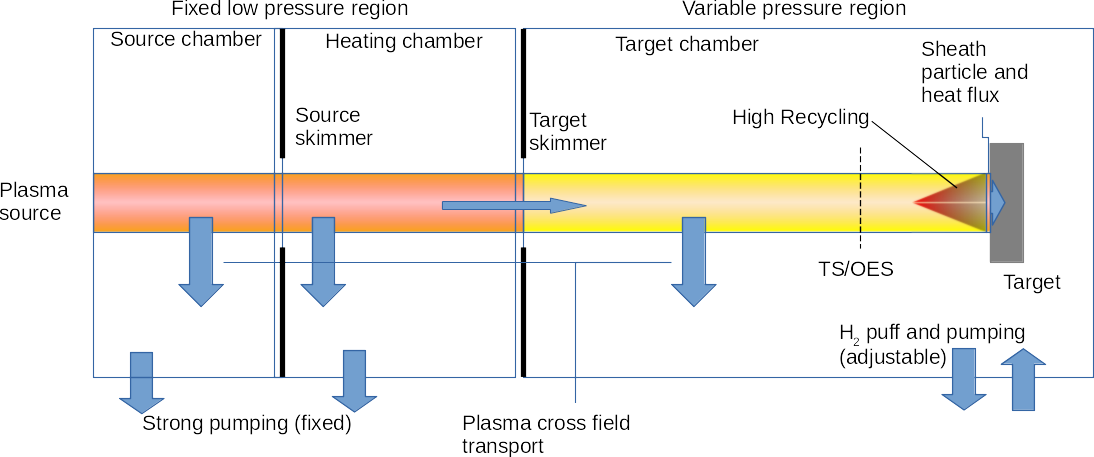
\includegraphics[width=\linewidth,trim={0 0 0 0},clip]{Chapters/chapter3/figs/plasma_column.png}
	\caption{Schematic of the plasma column model used. This schematic is useful to correlate local properties (at TS/OES location) to global ones like the total input power. Simplifications as constant densities and temperatures along the magnetic field and constant flow speed are used.}
	\label{fig:plasma_column1}
\end{figure*}

To avoid to consider precursor densities that could well match the line spectra but would lead to unrealistic power or particle losses a balance on the plasma column is performed. The definition of plasma column allows also to extract global information on the ELM-like pulse from the local TS/OES measurements and compare them with other global measurements like the power input from power supply. A schematic of the model of plasma column used is in \autoref{fig:plasma_column1}.

Fundamental assumptions are:
\begin{enumerate}
    \item Given the neutrals density in source and heating chamber is low thanks to differential pumping it is assumed that the plasma is transported undisturbed from the plasma source to the target skimmer. Here $T_e$,$n_e$ are equal to what is measured by TS in the target chamber for the lowest neutral pressure setting, that corresponds to the lowest possible volumetric losses.
    \item The plasma enters the target chamber without any molecular precursor. This is justified by the fact that from source to target chamber skimmer the neutral pressure is at it lowest while the temperature is at its highest and this conditions are the least favourable for reactions involving molecules.
    \item The neutral pressure is fixed throughout the ELM-like pulse to its steady state value.
    \item All plasma properties such as: temperatures, densities, reaction rates, radiated power, depend on radial and temporal coordinates only and are spatially constant from target skimmer to target. This is justified by the fact that the fast camera shows that in Stage 1 and 2 the radiation is mostly constant from a short distance off the target. Given the OES measuring location, only the properties of the bulk of the plasma can be analysed\footnote{Measurements specific to the region close to the target have been attempted but failed possibly due to reflections or obstructions by the target itself.}. That means that the power losses in the visible light brightness peak between the OES and the target observed in \autoref{Fast camera} cannot be accounted, so the volumetric power losses from the analysis will likely be an underestimation. The extent of the non uniform region close to the target, likely including sheath and strongly recycling region, is typically <1cm, small compared to the 38 cm from target to skimmer, so this underestimation should be minor. Increasing neutral pressure from Stage 1 to 2 (the cases we are most interested in) the visible light brightness becomes stronger in the plasma column, making the anisotropy at the target even less relevant. The approximation also neglects\ anisotropy in the visible light brightness in the bulk for very high neutral pressure. This is especially dominant in Stage 3, so it's importance should be minor for Stages 1 and 2.
    \item The plasma behaviour in the sheath and in the strongly recycling region is neglected.
    \item The flow velocity of the plasma is constant from the source to the target.
    \item Cross field transport is negligible (mostly true for charged particles due to the high magnetic field and additionally for molecular ions due to their short life time)
\end{enumerate}

Given these assumptions one can calculate the components of the power and particle balance on the whole plasma column. The OES/TS measurements from a single location can be applied to the whole column and the contribution from atomic and molecular processes can be found.

A quantity that will be used later is the flow velocity ($v_{in}$), the velocity of the plasma in its flow from the target skimmer to the target. It is here mainly used to subdivide the power from the plasma source (a global value) to what is provided to each radial location and to estimate the local particle inflow. It is also used to estimate the kinetic energy of the plasma, but the relevance of this term is minor. There is no direct measurement of $v_{in}$ yet as collective Compton scattering measurements will be available in the future. $v_{in}$ is then approximated by imposing, for the experimental condition with the lowest target chamber neutral pressure, that the power from the source matches the energy flow measured at the TS location. The flow is assumed having a single Mach number for all radial locations. Applying this conditions to \autoref{eq:plasma_column3} this translate to \autoref{eq:plasma_column1} that is then solved to find the Mach number.


\begin{equation}
\label{eq:plasma_column1}
\begin{aligned}
\sum_{r} \biggl\{ \biggl(\frac{1}{2} m_i v_{in}^2(r,t) +
&%\phantom{\biggr) \biggr\}} & \\ \phantom{\biggl\{ \biggl(}+
5k_B T_{e,in}(r,t) + E_{ion} + E_{diss} \biggr) \cdot \phantom{\biggr\}} & \\ \phantom{\biggl\{} \cdot n_{e,in}(r,t) v_{in}(r,t)A \biggr\} &= P_{source}(t)
\\
v_{in}(r,t) &= M_{in}(t) c_{s,up}(r,t) \\  c_s &= \sqrt{\frac{ \left(T_e + T_{H^+{}}( {}\approx T_e) \right)k_B}{m_H} }
\end{aligned}
\end{equation}

In calculating $P_{source}$ as product of voltage and current an efficiency of 92\% is considered in the conversion from electric to plasma energy.\cite{Morgan2014} $M_{in}$ is $\approx$1 during the ELM-like pulse. It must be noted that at the beginning and end of the pulse TS is incapable of accurately measuring across the whole plasma because of the low density, and the energy conversion from electric power to plasma potential is lower, resulting in the calculated $M_{in}>1$. The effect of the overestimation, though, is to allow for larger energy and particle budgets, widening the possible parameter space, so it is acceptable.
I will now detail how to calculate the likelihood associated with the power and particle balance.

\subsection{Power balance}\label{Power balance}

In this chapter it will be detailed how the power (energy) balance equation is obtained and how all the terms are defined.
The 1D energy and particle balance equations are obtained from the 1D Fokker-Planck collisional kinetic equation (\autoref{eq:plasma_column2}) as per derivation from Stangeby\cite{Verhaegh2021} and are adapted using the mentioned approximations for the region from target skimmer to target. This results for every time step and radial location in \autoref{eq:plasma_column3}
\begin{equation}
\label{eq:plasma_column2}
\begin{aligned}
  \frac{ \partial f }{ \partial t}  + v_z \frac{\partial f}{\partial z}  + \frac{eE}{m} \frac{ \partial f }{ \partial v_z} = \left( \frac{ \partial f }{ \partial t} \right)_{coll}  +  S(x,v)
\end{aligned}
\end{equation}
\begin{equation}
\label{eq:plasma_column3}
\begin{aligned}
\frac{  \partial E }{ \partial t} +& \frac{d}{dz}  \left[ \left( \frac{1}{2} m_i v^2 + 5kT_e + E_{ion} + E_{diss} \right) n_e v \right] =\\ -& \underbrace{P_{ext\ source}}_{= 0} + P_{ volume\ sinks-sources }
\\
\frac{  \partial E }{ \partial t} +& \left( \frac{1}{2} m_i v_{in}^2 + 5kT_{e,in} + E_{ion} + E_{diss} \right) n_{e,in} v_{in} =\\ &  + P_{ target } + P_{ volume\ sinks-sources }
\\
P_{diss \: max} =& \underbrace{ \left( \frac{1}{2} m_i v_{in}^2 + 5kT_e + E_{ion} + E_{diss} \right)  {\frac{n_e V}{\Delta t}}}_{P_{ \partial t}} + \\ &+ \underbrace{ \left( \frac{1}{2} m_i v_{in}^2 + 5kT_{e,in} + E_{ion} + E_{diss} \right) n_{e,in} v_{in}A}_{P_{in}} \geq \\ \geq & P_{ volume\ sinks-sources }
\end{aligned}
\end{equation}
with $v$ the flow velocity, $E_{ion}$ and $E_{diss}$ the ionisation and dissociation energy for hydrogen. The inequality arises from not accounting the power delivered to the target and to neglect plasma interactions with neutrals such as elastic collisions and charge exchange. All quantities marked with the subscript ${}_{in}$ refer to the input conditions, otherwise the conditions inside the plasma column are intended. $P_{\partial t}$ represents the power deriving by depleting all the energy associated with the plasma in the volume of interest ($V$) in a single time step ($\Delta t$), $P_{in}$ is the power entering the volume of interest from the plasma source through the area $A$. $P_{diss \: max}$ is the maximum power that can be depleted in a radial portion of the plasma column in a time step. As an additional constrain on the power balance it will be required to $P_{volume\ sink-source}$ to be positive, as otherwise it would mean that the plasma is externally heated on its way to the target.

Let’s investigate now the volumetric sinks-sources term. There are roughly three ways in which a hydrogen plasma can undergo power losses:
\begin{enumerate}
    \item Radiative losses. This mostly comes from the relaxation of excited hydrogen atoms, which can arise from both plasma-atom as well as plasma-molecule interactions. The radiative losses associated with $H_2$ molecular band radiation are expected to be of insignificant.\cite{Groth2019} \label{Radiative losses}
    \item Power transfer from kinetic energy to potential energy. Several plasma species have a relative potential energy associated with it (for instance, $H^+$ has a potential energy of 13.6eV compared to atomic hydrogen). Converting a neutral into an ion thus “converts” 13.6eV of kinetic plasma energy to potential energy.  \label{Power transfer potential}
    \item Power transfer from CX and elastic collisions. CX as well as elastic collisions between the plasma and neutral atoms and molecules can lead to transfer of power from the plasma to the neutrals (and vice versa). This includes collisions between particles of the same specie but at different temperatures like the cold proton generated from ionisation and the hot one part of the plasma. \label{Power transfer CX}
\end{enumerate}

OES combined with collisional radiative models is used to estimate the magnitude of both path \ref{Radiative losses} and \ref{Power transfer potential}, which is employed in this work. For path \ref{Radiative losses}, the Balmer line emission is measured facilitating, through the Bayesian inference of the plasma properties, a full estimate of the hydrogenic line radiation from excited atoms arising both from plasma-atom as well as plasma-molecule interaction. For path \ref{Power transfer potential}, ionisation and recombination rates are estimated to account for the power transfer between potential and kinetic energy. In the recombination reaction a hot $H^+$ is converted into a neutral. That neutral has a kinetic energy equal to the temperature of the plasma that generated it, significantly higher than all other molecular and neutral species. For this reason the energy removed by the plasma assuming the neutrals from recombination escape is accounted in the local power balance. Additionally a series of molecular reactions are considered, see \autoref{Reactions} for which the difference in potential energy between reactants and products is calculated and accounted.

Note that paths \ref{Power transfer potential} and \ref{Power transfer CX} do not strictly represent power lost from the plasma column but can be power transfer mechanisms. Such transfer mechanisms often lead to an effective loss of kinetic energy by the plasma, but can also cause it to increase.

In the power balance that regards the limitation of the power transferred from the plasma at a single radial location, \autoref{eq:plasma_column3}, pathway \ref{Power transfer potential} is considered. It is in fact impossible for the plasma to transfer energy from kinetic to potential for more more than it is available. Differently when the quantity of interest are the components of the global power balance, \autoref{eq:plasma_column9}, only terms where the energy is removed from the plasma column entirely will be considered. Internal power transfer will not be considered as it is energy that remains in the plasma.

Pathway \ref{Power transfer CX} cannot be readily analysed experimentally but can be analysed in detail in simulations. The importance of this is currently discussed in literature and it could be significant especially in low temperature conditions in tokamak divertors and linear machines. \cite{Myatra2021,Smolders2020,Chandra2022} Further code investigations on this and detailed comparisons against experiments are required, which is outside of the scope of this work. To check that neglecting CX and $H_2$ elastic collisions, the ones to have the largest impact\cite{Chandra2022}, does not have a negative impact on the consistency of the solution a crude estimation was done in post processing. This is done by first calculating the ADAS CCD reaction rate for CX and AMJUEL 3.5 rate for $H_2$ elastic. These are multiplied by the density of the reactant species interested and by the maximum energy that can be transfer with a single collision. The energy of the reactants are equivalent to their temperature from TS and \ref{Priors from B2.5 Eunomia}. This results in \autoref{eq:CX_elastic}.
\begin{equation}
\label{eq:CX_elastic}
\begin{aligned}
  P_{CX} &= \frac{ 3 }{ 2}  (T_{H^+}(=T_e)-T_H) RR_{CX}(T_e,n_e) n_{H^+} n_{H}
  \\
  P_{H_2 elastic} &= \frac{ 3 }{ 2} \frac{8}{9} (T_{H^+}-T_{H_2}) RR_{H_2 elastic}(T_{H^+},T_{H_2})  n_{H^+} n_{H_2}
\end{aligned}
\end{equation}
These quantities PDFs are calculated as one of the outputs of the Bayesian algorithm.

%The following is way too complicated. I simply do the product of the rates and that's it
%It is first calculated the inflow of $H_2$ from around the plasma towards the centre assuming sonic flow and the density arsing from the neutral pressure measurement. The consumption of $H_2$ is calculated and the fraction due to CX calculated with ADAS CCD coefficient. The atomic $H$ generated via CX is then assumed flowing outwards carrying the energy corresponding to the plasma temperature. The fraction of this atomic $H$ that undergo a reaction on the way out is then not accounted in the energy loss via CX. It is found that the total CX power loss is negligible respect to other terms. CX is relatively more relevant at low neutral pressure even if the neutral density is lower because the region with high temperature is wider and there is a higher chance of interaction between hot plasma and neutrals.

The sinks/sources terms for \autoref{eq:plasma_column3} are taken from different sources, to encompass the best knowledge available at the time of writing, see \autoref{Reactions}. Grouping them by type and precursor the power balance sinks/sources term is then defined as per \autoref{eq:plasma_column4}

\begin{equation}
\label{eq:plasma_column4}
\begin{aligned}
P_{ \substack{volume \\ sinks-sources}} =& P_{ radiated } + P_{ \substack{neutral\ via \\ recombination} } + P_{ potential\ energy }
\\
P_{ radiated } =& P_{ radiated\ atomic } + P_{ radiated\ molecular } 
\\
P_{ \substack{neutral\ via \\ recombination} } =& \frac{3}{2} \Delta V T_e RR_{rec}
\\
P_{ potential\ energy } =& \Delta V \sum_{i} { {\Delta E}_i \cdot RR_i } 
\\
P_{ radiated\ atomic } =& \underbrace{P_{ excitation }}_{ADAS\ PLT} + \underbrace{P_{ rec + bremsstrahlung }}_{ADAS\ PRB}
\\
P_{ radiated\ molecular } =& P_{ rad\ {H_2}^+{} } + P_{ rad\ {H_2} } + P_{ rad\ {H}^-{}+{H_2}^+{} } + \\ &+ P_{ rad\ {H}^-{}+{H}^+{} } + P_{ rad\ e^-{} + H \rightarrow {H}^-{}+hv } 
\\
P_{ rad,i } =& \Delta V \sum_{p=2,q<p}^{p=13} \epsilon^{i}_{pq}
\end{aligned}
\end{equation}

where $\Delta V$ represent the volume corresponding to the radial location of the plasma considered, $\Delta E_i$ is the energy difference between products and reactants of the reaction $i$ and $RR_i$ is its reaction rate. The ${}^{p=13}$ comes from the fact that only atomic hydrogen excited states up to 13 are here considered. The probability that the inequality in \autoref{eq:plasma_column3} is true and that $P_{volume\ sinks-sources}$ is positive is calculated with \autoref{eq:plasma_column5}
\begin{equation}
\label{eq:plasma_column5}
\begin{aligned}
y =& P_{diss \: max} - P_{s-s}, \sigma_{y} = \sqrt{{\sigma_{P_{\substack{s-s}}}}^2 + {\sigma_{P_{diss \: max}}}^2 }
\\
L_P =& L(y \in [0,P_{diss \: max}]) = \\ =& \frac{1}{2} \left[ erf ( \frac{P_{diss \: max}-y}{ \sqrt{2} \sigma_{y} }) - erf(\frac{-y}{ \sqrt{2} \sigma_{y} } ) \right]
\end{aligned}
\end{equation}
where $P_{volume\ sinks-sources}$ is shortened with $P_{s-s}$.

The power sinks/sources are calculated by adding all the radiative losses to the potential energy contribution. The latter is itself composed by positive and negative contributions that tend to cancel out. This causes the uncertainty of the sinks/sources to greatly dominate over the input one, making the effective use of this balance very difficult. To solve this issue $\sigma_y$ considered as equal to $\sigma_{\substack{P_{diss \: max}}}$ and that is assumed to be 50\% of $P_{diss \: max}$ (using the fixed nominal $T_e$, $n_e$ values from TS). 


\subsection{Particle balance}\label{Particle balance}

The derivation of the particle balance equation from Stangeby\cite{Stangeby2001} results in Equation 14

\begin{equation}
\label{eq:plasma_column6}
\begin{aligned}
\frac{ \partial n_j}{ \partial t} + \frac{d}{dz}   \left(n_j v \right) &= Sinks-Sources \\ (nv)_{j, diss \: max} &={\underbrace{\frac{n_j V }{ \Delta t }}_{(nv)_{j,\partial t}} + \underbrace{n_{j,in} v_{in}}_{(nv)_{j,in}}} \geq \\ \geq & (nv)_{j, Sinks-Sources} = \Delta V \sum_{i} f_{ij} RR_i 
\end{aligned}
\end{equation}

with $f_{ij}$ the multiplicity and sign in the reaction $i$ for the specie $j$ and ${n_{{H_2}}}_{in}={n_{{H}}}_{in}={n_{{H_2}^+}}_{in}={n_{H^-}}_{in} =0$. The inequality comes from not including the particles lost due to surface processes happening at the target and cross field transport. Charged particles are bound by magnetic fields while neutrals can more easily move across. For this reason the particle balance, that considers each radial location independently, is calculated only for charged particles as $e^-$, $H^+$, ${H_2}^+$, $H^-$.
In the case of ${H_2}^+$, $H^-$ the lifetime is very short so even in a single time step it is not physical to allow for its accumulation. For this reason for them $(nv)_{i, Sinks-Sources}$ is limited to be $\geq -(nv)_{i, diss \: max}$. For $e^-$ and $H^+$ the net rate of production is limited to their density the next time step. This term, referred as $(nv)_{j,next}$ is defined similarly to $(nv)_{j,\partial t}$ in \autoref{eq:plasma_column6}. The likelihood that the particle balance is verified is given by \autoref{eq:plasma_column7a} and \ref{eq:plasma_column7b}

\begin{equation}
\label{eq:plasma_column7a}
\begin{aligned}
y_j &= (nv)_{j, diss \: max} - (nv)_{j, Sinks-Sources} \\ {\sigma}_{y_j} &=\sqrt{{{\sigma}_{(nv)_{j, diss \: max}}}^2 + {{\sigma}_{(nv)_{j, Sinks-Sources}}}^2 }
\\
L\left(y_{e^-{}} \in \right. & \left. [0,(nv)_{e^-, diss \: max}+(nv)_{e^-, next}]\right) =\\=& \frac{1}{2} \left[ erf \left(\frac{(nv)_{e^-, diss \: max}+(nv)_{e^-, next}-y_{e^-}}{\sqrt{2} {\sigma}_{y_{e^-}} } \right) \right. +\\ &-\left. erf \left( \frac{-y_{e^-{}}}{\sqrt{2} {\sigma}_{y_{e^-{}}} } \right) \right]
\\
L\left(y_{H^+{}} \in \right. & \left. [0,(nv)_{H^+{}, diss \: max}+(nv)_{H^+{}, next}]\right) =\\=& \frac{1}{2} \left[ erf \left(\frac{(nv)_{H^+{}, diss \: max}+(nv)_{H^+{}, next}-y_{H^+{}}}{\sqrt{2} {\sigma}_{y_{H^+{}}} } \right) \right. +\\ &-\left. erf \left( \frac{-y_{H^+{}}}{\sqrt{2} {\sigma}_{y_{H^+{}}} } \right) \right]
\end{aligned}
\end{equation}

\begin{equation}
\label{eq:plasma_column7b}
\begin{aligned}
L\left(y_{{H_2}^+{}} \in \right. & \left. [0,2(nv)_{{H_2}^+{}, diss \: max}]\right) = \\ =& \frac{1}{2} \left[ erf \left(\frac{2(nv)_{{H_2}^+{}, diss \: max}-y_{{H_2}^+{}}}{\sqrt{2} {\sigma}_{y_{{H_2}^+{}}} } \right) \right. +\\ &-\left. erf \left(\frac{-y_{{H_2}^+{}}}{\sqrt{2} {\sigma}_{y_{{H_2}^+{}}} } \right) \right]
\\
L\left(y_{{H}^-{}} \in \right. & \left. [0,2(nv)_{{H}^-{}, diss \: max}]\right) = \\ =& \frac{1}{2} \left[ erf\left(\frac{2(nv)_{{H}^-{}, diss \: max}-y_{{H}^-{}}}{\sqrt{2} {\sigma}_{y_{{H}^-{}}} } \right) \right. +\\ &- \left. erf\left(\frac{-y_{{H}^-{}}}{\sqrt{2} {\sigma}_{y_{{H}^-{}}} } \right) \right]
\\
L_{nv} &= L(y_{e^-{}} \geq 0) \cdot L(y_{H^+{}} \geq 0) \cdot \\ & \phantom{=} \cdot L(y_{{H_2}^+{}} \in [0,2(nv)_{{H_2}^+{}, diss \: max}]) \cdot \\ & \phantom{=} \cdot L(y_{{H}^-{}} \in [0,2(nv)_{{H}^-{}, diss \: max}]) 
\end{aligned}
\end{equation}

Similarly to what mentioned for the power balance, here too the sinks/sources term is composed of positive and negative factor, so rather than using it a large uncertainty on $(nv)_{i, diss \: max}$ of 100\% for $e$, $H^+$ (using the fixed nominal $n_e$ value from TS) and 5\% of TS $n_e$ for ${H_2}^+$, $H^-$ is assumed. The uncertainties are here adopted so large because differently from power and emissivity there is no direct measurement of the particle input.
As part of the particle balance one has also to include that the density of excited states obtained with ADAS and Yacora coefficients is lower than the density of total atomic hydrogen in the volume. This is calculated with \autoref{eq:plasma_column8}.

\begin{equation}
\label{eq:plasma_column8}
\begin{aligned}
y = n_{H} - \sum_{q,i} n_{i H(q)}, \sigma_{y} = \sqrt{ \sum_{q,i} (\sigma_i n_{i H(q)})^2  }
\\
L_{H^{exc}} = L(y \geq 0) = \frac{1}{2} \left[ 1 - erf\left(\frac{-{y}}{ \sqrt{2} \sigma_{y} } \right) \right]
\end{aligned}
\end{equation}

\subsection{Plasma column power balance}\label{Plasma column power balance}

The definition of the plasma column volume and the power balance allows to evaluate the global performance of the detached target to the ELM-like pulse. The parameter of interest is, in this case, how much power is removed from the plasma column and how much is due to atomic versus molecular effects.
In considering this the potential energy exchange due to EIR, for example, was not considered because it represent a transfer mechanism and not a net loss, while the radiative component due to radiation (ADAS PRB coefficient, returning the losses due to line radiation and Bremsstrahlung) was. Bremsstrahlung radiation is present also in the wavelength range of the IR camera and could be related to the observed prompt emission but this was not investigated. Similarly all other exchanges of potential energy are not considered. The generated neutrals while travelling out of the plasma can react with the neighbouring plasma and the energy they carry be reintroduced. Because evaluating this would require a significant effort this component is for now excluded.

The terms considered for the global power removed from the plasma column are indicated in \autoref{eq:plasma_column9}.
\begin{equation}
\label{eq:plasma_column9}
\begin{aligned}
 E_{ \substack{removed \\ from \\ plasma}} = E_{ radiated } =& \underbrace{E_{exc} + E_{rad\ rec+bremm}}_{atomic} +\\&+ E_{rad\ {H_2} } + E_{rad\ {H}} + E_{rad\ {H_2}^{+{}} } +\\& \underbrace{ +E_{rad\ {H}^{-{}} } + E_{rad\ e^-{}+H \rightarrow {H}^{-{}}+pv \phantom{+}}}_{ molecular }
\end{aligned}
\end{equation}
Once all the likelihoods associated with each combination of priors are calculated they are multiplied to return the total likelihood as per \autoref{eq:plasma_column10}

\begin{equation}
\label{eq:plasma_column10}
\begin{aligned}
L = P_{\epsilon} L_p L_{nv} L_{H^{exc}}
\end{aligned}
\end{equation}

The PDFs of all the components of the power and particle balance previously calculated are built by portioning their range to a smaller number of logarithmic intervals, summing the probability within. For each additive term of interest the PDFs are then convolved in space and in time to obtain the PDF for the whole ELM-like pulse. For each radial and time location and for each output required (for example the total radiated energy) is defined a large list of the possible energy losses in that section of the plasma. The list is randomly distributed according on the PDF of that output at that location. The contribution for all radii is summed to generate a list of possible values of the total radiated energy at one time step. A histogram is built based on that to represent the PDF of the quantity of interest at that time step. This operation is repeated to sum the contribution from all the time steps to return the PDF of the quantity of interest for the whole ELM-like pulse.

\subsection{Reactions}\label{Reactions}

Reaction rates and other coefficients used in the Bayesian calculations are obtained from ADAS\cite{Summers2004,OMullane2013} for the atomic reactions while from Yacora \cite{Wunderlich2016,Wunderlich2020}, AMJUEL\cite{Reiter2017,Reiter2005,Kotov2007} %ALADDIN\cite{IAEANuclearDataSection}
or a collection of reaction rates from Janev\cite{Janev2003} for the molecular reactions. The reactions considered in this work are listed in \autoref{tab:adas}, \ref{tab:yacora}, \ref{tab:amjuel}, %\ref{tab:aladdin}
and \ref{tab:janev}.

\begin{table}[h]
\begin{tabular}{ | p{7cm}| m{3.5cm} | } 
\hline
Reaction: & Chapter / type \\ 
\hline
$H^+ + e^- \rightarrow H(p) + h\nu$ \newline $H^+ + 2e^- \rightarrow H(p) + e^-$ & ADC,PRB,PEC \\ 
\hline
$H + e^- \rightarrow H^+ + 2e^-$ & SCD \\
\hline
$H(q) + e^- \rightarrow H(p>q) + e^-$ & PLT,PEC\\
\hline
\end{tabular}
\caption{Reactions whose rates and reference coefficients were sourced from the ADAS database.\cite{Summers2004,OMullane2013}}
\label{tab:adas}
\end{table}

\begin{table}[h]%[ht!]
\begin{tabular}{ | p{7cm}| m{3.5cm} | } 
\hline
Reaction: & Chapter / type \\ 
\hline
${H_2}^+ + H^- \rightarrow H(p) + H_2$ &  \\
\hline
$H^+ + H^- \rightarrow H(p) + H$ & \\
\hline
${H_2}^+ + e^- \rightarrow H(p) + H(1)$ & \\
\hline
${H_2}^+ + e^- \rightarrow H(p) + H^+ + e^-$ & \\
\hline
$H_2 + e^- \rightarrow H(p) + H(1) + e$ & \\
\hline
\end{tabular}
\caption{Reactions whose rates and reference coefficients were sourced using the Yacora collisional radiative code.\cite{Wunderlich2016,Wunderlich2020}}
\label{tab:yacora}
\end{table}

\begin{table}[h]
\begin{tabular}{ | p{7cm}| m{3.5cm} | } 
\hline
Reaction: & Chapter / type \\ 
\hline
$e^- + H_2 \rightarrow 2e^- + {H_2}^+$ & 4.11 Reaction 2.2.9 \\
\hline
$e^- + H_2 \rightarrow 2e^- + H + H^+$ & 4.12 Reaction 2.2.10 \\
\hline
$e^- + {H_2}^+ \rightarrow 2e^- + H^+ + H^+$ & 4.13 Reaction 2.2.11 \\
\hline
$e^- + {H_2}^+ \rightarrow e^- + H + H^+$ & 4.14 Reaction 2.2.12 \\
\hline
$e^- + {H_2}^+ \rightarrow H + H$ & 4.15 Reaction 2.2.14 \\
\hline
$e^- + H_2 \rightarrow e^- + H_2(v) \rightarrow H + H^-$ & 2.23 Reaction 2.2.17 \\
\hline
$H^+ + H_2(v) \rightarrow H + {H_2}^+$ & 3.28 Reaction 3.2.3 \\
\hline
$H^+ + H^- \rightarrow H + H$ & 4.52 Reaction 7.2.3a \\    % this one CANNOT be deleted as a reaction in Yacora too
\hline
$e^- + H_2(v) \rightarrow e^- + H + H$ & 4.10 Reaction 2.2.5g \\    % this one CANNOT be deleted as a reaction in Yacora too
\hline
\end{tabular}
\caption{Reactions whose rates and reference coefficients were sourced from the AMJUEL database.\cite{Reiter2017,Reiter2005,Kotov2007}}
\label{tab:amjuel}
\end{table}

% \begin{table}
% \begin{tabular}{ | p{5.5cm}| m{2.8cm} | } 
% \hline
% Reaction: & Chapter / type \\ 
% \hline
% neglected because very uncertain rate
%${H_2}^+(1s\sigma g;v=0-9) + H(1) \rightarrow $\newline $\rightarrow H^+ + H(1) + H(1)$ & Reaction rate \\
%\hline
% neglected because very uncertain rate
%$H(1) + H(3) \rightarrow {H_2}^+(v) + e^-$ & Cross section \\
%\hline
% neglected because very uncertain rate
%$e^- + H^- \rightarrow e^- + H + e^-$ & Reaction rate \\
%\hline
% neglected because very uncertain rate
%$H^- + H_2(v) \rightarrow H + H_2(v") + e^-$ & Cross section \\
% \hline
% \end{tabular}
% \caption{Reactions whose rates and reference coefficients were sourced from the iaea.org/ALADDIN database}
% \label{tab:aladdin}
% \end{table}

\begin{table}[h]
\begin{tabular}{ | p{7cm}| m{3.5cm} | } 
\hline
Reaction: & Chapter / type \\ 
\hline
% neglected because very uncertain rate
%${H_2}^+(vi) + H_2(v0) \rightarrow ({H_3}^+* + H) \rightarrow $\newline $\rightarrow H^+ + H + H_2(v01)$ \newline ${H_2}^+(vi) + H_2(v0) \rightarrow $\newline $\rightarrow [{H_2}^+(2p\sigma u/2p\Pi u···) + H_2] \rightarrow $\newline $\rightarrow H^+ + H + H_2(v01)$ & 7.3.2 \\
%\hline
% neglected because very uncertain rate
%$H^+ + H^- \rightarrow {H_2}^+(v) + e^-$ & 3.2.2 \\
%\hline
% neglected because very uncertain rate
%$H^+ + H(1) + H(1) \rightarrow H^+ + H_2(\nu)$ & 2.2.4, equation 46a \\
%\hline
% neglected because very uncertain rate
%$H^+ + H(1) + H(1) \rightarrow H(1) + {H_2}^+(\nu)$ & 2.2.4, equation 46b \\
%\hline
% neglected because very uncertain rate
%$H(1) + H(2) \rightarrow {H_2}^+(v) + e^-$ & 2.3.3 \\
%\hline
% neglected because very uncertain rate
%$H(1) + H(4) \rightarrow {H_2}^+(v) + e^-$ & 2.3.3 \\
%\hline
% neglected because very uncertain rate
%$H+H+H \rightarrow H_2 + H$ & 2.3.4 \\
%\hline
% neglected because very uncertain rate
%$H^- + H(1) \rightarrow {H_2}^-(B2\Sigma+g) \rightarrow $\newline $\rightarrow H(1) + H(1) + e^-$ & 3.3.2 \\
%\hline
% neglected because very uncertain rate
%$H^- + H(1) \rightarrow {H_2}^-(X2\Sigma+u;B2\Sigma+g) \rightarrow $\newline $\rightarrow {H_2}(X1\Sigma+g,v) + e^-$ & 3.3.2 \\
% neglected because very uncertain rate
%$H^+ + H_2(X1\Sigma+g,v) \rightarrow H^+ + H(1) + H(1)$ & 5.3 \\
% neglected because very uncertain rate
%$H(1) + H_2(v) \rightarrow H(1) + H(1) + H(1)$ & 6.2.2 \\
%\hline
% neglected because very uncertain rate
%$H_2(v=0) + H_2(v) \rightarrow H_2(v=0) + H(1) + H(1)$ & 6.3.2 \\
%\hline
% neglected because very uncertain rate
%$e^- + H(1) \rightarrow H^- + h\nu$ & 2.1.3 \\
%\hline
${H_2}^+(vi) + H^- \rightarrow ({H_3}^*) \rightarrow $\newline $\rightarrow H_2(X1\Sigma_g;v_0) + H(n\geq 2)$ & 7.4.1 \\    % this one CANNOT be deleted as a reaction in Yacora too
\hline
${H_2}^+(vi) + H^- \rightarrow ({H_3}^*) \rightarrow $\newline $\rightarrow H_2(N1,3\Lambda_{\sigma};v_0) + H(1),N \leq 4$ & 7.4.1 \\   % this one CANNOT be deleted as a reaction in Yacora too
\hline
\end{tabular}
\caption{Reactions whose rates and reference coefficients were sourced from the Janev database.\cite{Janev2003}}
\label{tab:janev}
\end{table}



